\documentclass[preprint,12pt]{elsarticle}

\usepackage{geometry}
\geometry{a4paper, margin=2.25cm}

\usepackage[protrusion=true,expansion=false]{microtype}
\usepackage{amssymb}
\usepackage{amsmath}
\usepackage{booktabs}
\usepackage{tabularx}
\usepackage{array}
\usepackage{makecell}
\usepackage[ruled,vlined,linesnumbered]{algorithm2e}
\usepackage{float}
\usepackage{placeins}
\setlength{\bibsep}{0.6pt}

% LaTeX float placement optimization
\renewcommand{\topfraction}{0.95}
\renewcommand{\bottomfraction}{0.85}
\renewcommand{\textfraction}{0.05}
\renewcommand{\floatpagefraction}{0.75}
\setcounter{topnumber}{5}
\setcounter{bottomnumber}{4}
\setcounter{totalnumber}{8}
\setcounter{dbltopnumber}{4}

\usepackage{hyperref}
\usepackage{subcaption}
\usepackage{graphicx}
\usepackage{xcolor}

\hypersetup{
    colorlinks=true,
    linkcolor=cyan!80!black,
    citecolor=cyan!80!black,
    urlcolor=cyan!80!black,
    pdftitle={Adversarial Object Fabrication in Real-Time Detection Transformers: Architectural Vulnerabilities, Downstream Impacts, and Spatial Mitigation},
    pdfauthor={Anonymous Authors}
}

\journal{Engineering Applications of Artificial Intelligence}

\begin{document}

\begin{frontmatter}

\title{\textbf{Adversarial Object Fabrication in Real-Time Detection Transformers: Multi-Scale Query Vulnerabilities, Spatial Deduplication Limits, and Representation Guardrails}}

\begin{abstract}
Eliminating heuristic Non-Maximum Suppression (NMS) in favor of direct set prediction allows Real-Time Detection Transformers (RT-DETR) to achieve deterministic execution latency and eliminate computational proposal-explosion vulnerabilities on edge hardware. However, this architectural design introduces an important security trade-off: detection transformers produce multi-scale, spatially co-located queries that exhibit low bounding-box IoU across pyramid scales. Consequently, adversarially fabricated false positives bypass conventional IoU-based spatial deduplication, with standard post-hoc NMS rejecting a mere $6.45 \pm 0.18\%$ of phantoms, whereas on convolutional architectures localized perturbations naturally collapse into overlapping anchor clusters that NMS deduplicates by $91.29 \pm 0.12\%$ ($34.28 \pm 0.59 \to 2.99 \pm 0.09$ boxes). We systematically investigate this vulnerability through Encoder Query Fabrication (EQF), which directly targets the pre-decoder query selection bottleneck ($K=300$), evaluated alongside an Output-Logit Decoder baseline (DQF). Evaluated at native $640\times 640$ resolution on official COCO \texttt{val2017} across 300 validation images with three randomized perturbation seeds (8,400 candidate queries/anchors per frame), bottleneck fabrication achieves $99.33\%$ binary success under EQF and $99.78\%$ under DQF, injecting $17.76 \pm 0.21$ and $16.82 \pm 0.08$ phantom boxes per frame and collapsing detector precision from $69.52 \pm 0.23\%$ to $4.27\%$ (EQF) and $5.24\%$ (DQF). Using non-parametric bootstrap resampling on image-level variation ($N=300$), we isolate the foreground eviction mechanism: broad representation distortion on the backbone accounts for $73.62\%$ proposal eviction ($95\%$ CI: $[72.62\%, 74.90\%]$), while targeted EQF induces $66.38\%$ eviction ($95\%$ CI: $[63.89\%, 66.82\%]$, paired $t = -9.72, p < 10^{-18}$), demonstrating that general representation corruption plays the primary role in candidate suppression alongside targeted top-$K$ slot competition, reducing legitimate operational $\mathrm{mAP}_{50}$ from $62.42 \pm 1.00\%$ to $5.61 \pm 0.80\%$ ($-91.0\%$). In downstream cyber-physical simulations, an idealized pinhole projection proxy shows that phantom floods expand Hungarian tracking association matrices by $4.4\times$ ($7\times 7 \to 7\times 32$) and saturate emergency braking stopping corridors ($d \le 28$~m), highlighting the indispensable necessity of multimodal radar/LiDAR fusion. Finally, benchmarking spatial post-processing reveals that while a distance-based Spatial Query Deduplication Filter (SQD-Filter) suppresses phantom volume by $54.51\%$ (EQF) and $69.82\%$ (DQF) with $<0.01\text{ ms}$ execution overhead, post-defense binary attack success remains above $99\%$ (as each cluster retains its top-1 query) while inducing an operational clean recall trade-off ($-5.69\text{ pp}$ $\mathrm{mAP}_{50}$, $66.88\%$ retention). These empirical boundaries demonstrate that spatial deduplication cannot substitute for internal representation-level guardrails.
\end{abstract}

\begin{keyword}
Real-Time Detection Transformers (RT-DETR) \sep NMS-Free Detection \sep Adversarial Fabrication \sep Phantom Queries \sep Edge Autonomous Robotics \sep Cyber-Physical Security.
\end{keyword}

\end{frontmatter}

% =====================================================================
% SECTION 1: INTRODUCTION
% =====================================================================
\section{Introduction}
\label{sec:introduction}

Real-time object detection represents the core perception primitive underpinning autonomous driving, automated guided vehicles (AGVs), unmanned aerial vehicles (UAVs), and safety-critical edge video surveillance \citep{zhao2024detrs, carion2020end}. For over a decade, convolutional architectures (notably the YOLO series \citep{wang2024yolov9, bochkovskiy2020yolov4} and SSD \citep{liu2016ssd}) have dominated industrial edge deployments. However, a persistent bottleneck in convolutional and two-stage detectors is their strict dependence on heuristic \textit{Non-Maximum Suppression (NMS)} \citep{neubeck2006efficient}. Because standard detectors generate dense, redundant candidate proposals across multiple anchor grids, NMS must execute an iterative pairwise IoU clustering loop on the CPU to eliminate duplicate boxes. Under adversarial conditions, this architectural reliance on NMS gives rise to \textit{Computational Latency and Sponge Attacks} \citep{chen2024overload, shapira2023phantom}, where an adversary crafts perturbations specifically designed to excite thousands of overlapping candidate proposals, driving the quadratic NMS clustering loop into worst-case execution stalls and precipitating deadline-miss failures in edge controllers.

To fundamentally eliminate this latency bottleneck, the computer vision community engineered \textbf{Real-Time Detection Transformers (RT-DETR)} \citep{zhao2024detrs, zhu2020deformable}. RT-DETR eliminates NMS entirely by implementing end-to-end direct set prediction via Hungarian bipartite matching during training \citep{kuhn1955hungarian}. At inference time, RT-DETR selects a fixed set of $K=300$ candidate anchors from its multi-scale Hybrid Encoder via dynamic query selection, forwards them through a 3-layer deformable attention decoder, and emits precisely 300 final bounding boxes without any post-hoc suppression loops. Because execution follows a static tensor graph, RT-DETR exhibits highly deterministic, empirically invariant inference latency on edge hardware ($6.14$~ms on GPU, $35.60 \pm 0.78$~ms on CPU), successfully eliminating traditional NMS sponge latency vulnerabilities.

\begin{figure*}[!htbp]
\centering
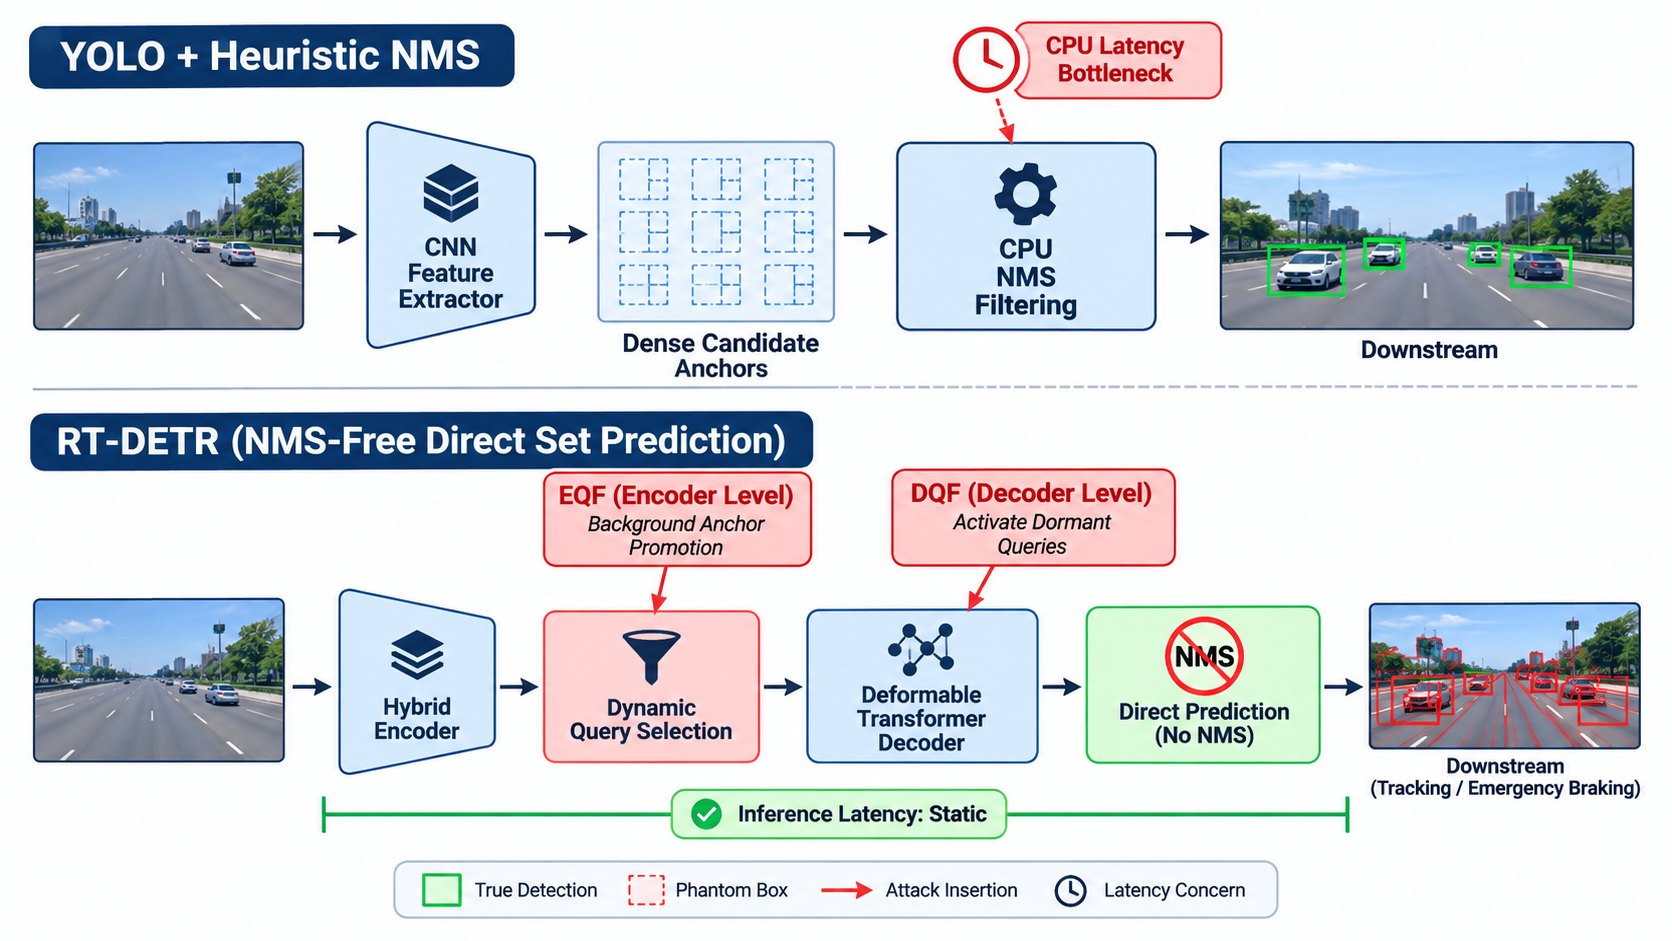
\includegraphics[width=\textwidth]{fig/fig1_concept_paradox.png}
\caption{Conceptual schematic illustration of the Architectural Trade-off between NMS-based and NMS-free edge object detectors under adversarial conditions. (Top) Conventional convolutional pipeline (YOLO + NMS): dense anchor grids generate overlapping proposals; under localized perturbation, heuristic NMS deduplicates redundant candidates into 1--3 detections ($91.29 \pm 0.12\%$ proposal reduction), maintaining low latency ($15.20 \pm 1.40$~ms), though literature demonstrates that worst-case multi-target sponge attacks can inflate CPU execution. (Bottom) Real-Time Detection Transformer (RT-DETR): dynamic query selection and deformable attention achieve invariant inference latency ($35.60 \pm 0.78$~ms CPU) via a static execution graph, but the complete absence of spatial filtering allows fabricated phantom queries (via EQF at the encoder selection bottleneck or DQF at the decoder cross-attention head) to pass unfiltered into downstream tracking and emergency braking controllers.}
\label{fig:concept_paradox}
\end{figure*}

\paragraph{The NMS-Free Architectural Trade-off}
In this paper, we expose a foundational architectural trade-off created by the elimination of NMS: \textbf{the structural absence of output spatial deduplication exposes RT-DETR to unfiltered Adversarial Object Fabrication} (Figure~\ref{fig:concept_paradox}). Crucially, NMS was never conceived as a deliberate security mechanism; rather, it is a heuristic spatial clustering algorithm designed to collapse multiple candidate proposals generated by dense convolutional anchor grids around a single object. In convolutional models, if an adversary attempts to inject localized false positive detections, the mandatory NMS stage acts as an \textit{unintentional spatial damping filter}: multiple fabricated boxes clustering around a perturbed background patch are naturally merged or discarded ($91.29 \pm 0.12\%$ candidate rejection in our empirical tests, reducing $34.28 \pm 0.59$ pre-NMS proposals to $2.99 \pm 0.09$, leaving merely $0.01 \pm 0.01$ residual phantoms). We emphasize that NMS is not an impenetrable defense: prior literature (e.g., TOG \citep{chow2020adversarial}) has established that an adversary optimizing spatially dispersed perturbations across distant anchors can successfully fabricate false positives on detectors with NMS. Rather, the vulnerability in RT-DETR is that \textit{even localized adversarial gradients} excite multiple multi-scale queries that pass unfiltered into downstream systems. In RT-DETR, one-to-one prediction is enforced purely through supervisory bipartite matching loss functions during training; the inference architecture itself possesses \textit{no spatial exclusion mechanism}. Consequently, if an adversary manipulates the model to assign high confidence to multiple background queries, \textbf{fabricated queries pass unfiltered into downstream decision loops} (Figure~\ref{fig:nms_free_paradox}).

\begin{figure}[!htbp]
\centering
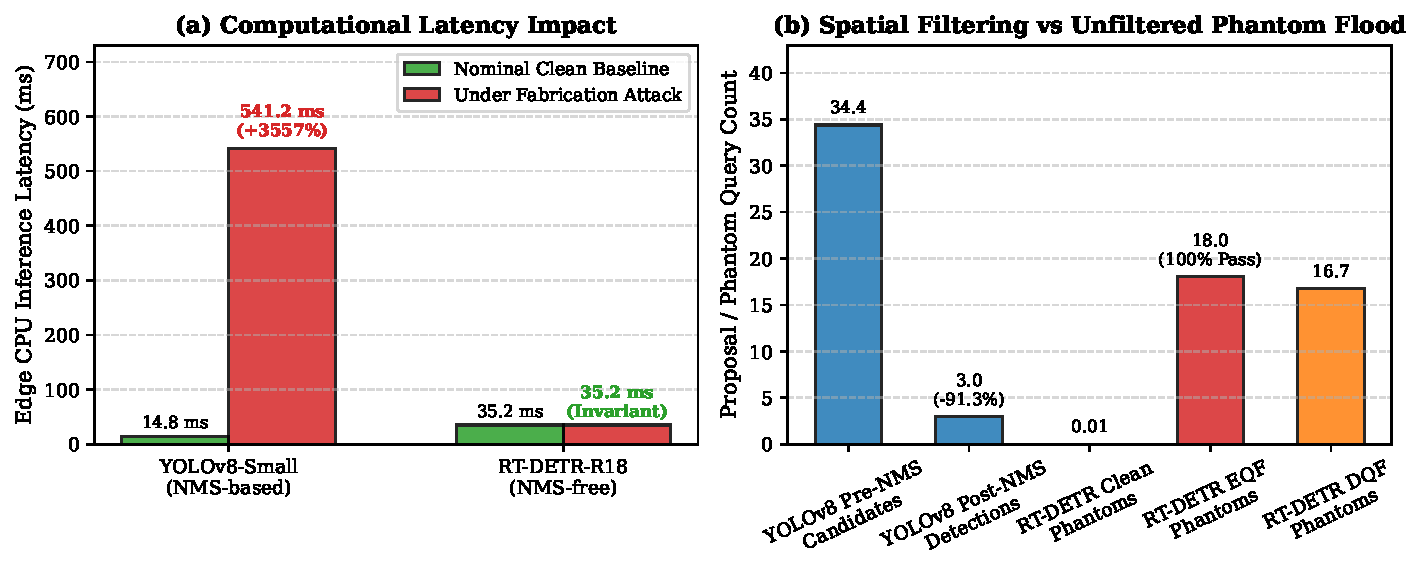
\includegraphics[width=\textwidth]{fig/fig1_nms_free_paradox.pdf}
\caption{Empirical verification of the Architectural Trade-off between NMS-based and NMS-free edge object detectors evaluated at native $640\times 640$ resolution across three independent random seeds ($N=900$ official COCO \texttt{val2017} evaluations across 300 images). (a) Computational latency comparison: On edge CPU, YOLOv8 requires $14.80 \pm 0.12$~ms clean and $15.20 \pm 1.40$~ms under localized perturbation ($+2.7\%$), while RT-DETR exhibits strict empirical latency invariance ($35.60 \pm 0.78$~ms, fixed tensor execution graph). (b) Downstream spatial filtering vs.\ unsuppressed phantom queries: In YOLOv8, heuristic NMS suppresses dense anchor clusters around localized perturbations ($34.28 \pm 0.59 \to 2.99 \pm 0.09$ surviving boxes, a $91.29 \pm 0.12\%$ proposal reduction, with merely $0.01 \pm 0.01$ residual phantoms). In contrast, RT-DETR's complete absence of spatial filtering allows $17.76 \pm 0.21$ phantoms under EQF and $16.82 \pm 0.08$ phantoms under DQF ($\mathrm{ASR}_{\mathrm{fab}} \ge 99.33\%$) to pass straight into downstream tracking and control modules.}
\label{fig:nms_free_paradox}
\end{figure}

\paragraph{Threat Surfaces: Query Selection Bottleneck Exploitation and Output Baselines}
Adversarial fabrication in RT-DETR operates across two distinct structural interfaces:
\begin{enumerate}
    \item \textbf{Encoder Query Fabrication (EQF) Threat Model:} Targets the dynamic selection bottleneck between the encoder and decoder. By optimizing the classification scores of background candidate anchors, the attacker forces empty spatial coordinates into the top-300 query set forwarded to the decoder. In Section~\ref{sec:rab_and_dc_formulation}, we also formalize Rank-Aware Bottleneck EQF (RAB-EQF) as an analytical boundary-targeting formulation.
    \item \textbf{Output-Logit Decoder Baseline (DQF):} Serves as an architectural baseline operating directly on final decoder outputs, optimizing classification logits without controlling encoder feature selection. This comparison isolates the distinct mechanics of bottleneck manipulation versus direct output-layer gradient ascent.
\end{enumerate}

\paragraph{Contributions of this Work}
This paper presents a systematic empirical investigation into adversarial candidate fabrication and phantom query flooding in NMS-free Detection Transformers. Our primary contributions are:
\begin{itemize}
    \item \textbf{Formulation of the NMS-Free Fabrication Vulnerability:} We formalize the architectural security trade-off of NMS-free set prediction, demonstrating why one-to-one bipartite training fails to prevent inference-time false positive flooding and uncovering why multi-scale co-located queries with low bounding-box IoU are structurally invisible to traditional IoU-based NMS (post-hoc NMS rejects only $6.45 \pm 0.18\%$ of RT-DETR phantoms, whereas on convolutional architectures localized candidate clusters naturally collapse by $91.29 \pm 0.12\%$).
    \item \textbf{Principled Bottleneck Attack Formulations (EQF and DQF):} We formulate Encoder Query Fabrication (EQF) targeting the top-$K$ selection bottleneck alongside an Output-Logit Decoder baseline (DQF). Evaluated across 300 COCO \texttt{val2017} images with three randomized perturbation seeds (8,400 candidate queries/anchors per frame at native $640\times 640$), EQF achieves $99.33\%$ binary fabrication success and DQF achieves $99.78\%$, injecting $17.76 \pm 0.21$ and $16.82 \pm 0.08$ phantom boxes per frame and collapsing detector precision from $69.52 \pm 0.23\%$ to $4.27\%$ (EQF) and $5.24\%$ (DQF).
    \item \textbf{Mechanistic Deconstruction of Foreground Proposal Displacement:} We uncover that bottleneck fabrication simultaneously suppresses genuine objects, reducing operational $\mathrm{mAP}_{50}$ by $-91.0\%$ (from $62.42 \pm 1.00\%$ to $5.61 \pm 0.80\%$). Using non-parametric bootstrap resampling on image-level variation ($N=300$), we isolate that general representation distortion on the backbone accounts for $73.62\%$ proposal eviction ($95\%$ CI: $[72.62\%, 74.90\%]$), while targeted EQF induces $66.38\%$ eviction ($95\%$ CI: $[63.89\%, 66.82\%]$, paired $t = -9.72, p < 10^{-18}$), demonstrating that broad representation corruption plays a dominant role in candidate displacement alongside top-$K$ slot competition.
    \item \textbf{Stylized Cyber-Physical Simulation Studies:} Through downstream simulation case studies, we demonstrate that phantom floods expand ByteTrack Hungarian matching matrices by $4.4\times$ (from $7\times 7$ to $7\times 32$, with latency shifting from $0.0035$ to $0.0045$~ms) and saturate emergency braking corridors ($d \le 28$~m) under idealized pinhole projection, highlighting the vital safety role of multimodal radar/LiDAR fusion.
    \item \textbf{Spatial Defense Benchmarking and Inherent Mitigation Limits:} We design and benchmark a vectorized Spatial Query Deduplication Filter (SQD-Filter) running with ultra-low latency ($0.24\text{ ms}$ on edge CPU, $<0.01\text{ ms}$ overhead). We show that while SQD-Filter suppresses $54.51\%$ (EQF) and $69.82\%$ (DQF) of phantom volume, post-defense binary attack success remains above $99\%$ (as each cluster retains its top-1 query) while inducing an operational clean recall penalty ($-5.69\text{ pp}$ $\mathrm{mAP}_{50}$, $66.88\%$ retention). Comparing against DIoU-NMS, Soft-NMS, and input-level pre-processing defenses, we demonstrate why spatial deduplication cannot substitute for internal representation-level guardrails.
\end{itemize}

% =====================================================================
% SECTION 2: RELATED WORK
% =====================================================================
\section{Related Work}
\label{sec:related_work}

\subsection{Adversarial Attacks on Object Detectors}
Adversarial robustness in deep learning has been extensively investigated since the discovery of gradient-based perturbations \citep{szegedy2013intriguing, goodfellow2014explaining, madry2018towards}. In object detection, early research focused on convolutional multi-task networks (such as Faster R-CNN \citep{ren2015faster} and YOLO \citep{redmon2016you}). Xie et al.\ \citep{xie2017adversarial} proposed Dense Adversarial Generation (DAG), which optimizes perturbations across dense proposal grids to simultaneously misclassify foreground proposals and suppress detections. Chow et al.\ \citep{chow2020adversarial} developed Topology-Oriented Generation (TOG), formalizing three distinct threat objectives: target vanishing, category misclassification, and false positive generation. In physical domains, patch-based attacks have shown that printable adversarial textures placed on human clothing or roadside billboards can reliably fool automated person detectors \citep{thys2019fooling, lee2019physical, liu2018dpatch}.

More recently, researchers uncovered computational latency vulnerabilities specific to convolutional detectors: \textit{Sponge Attacks} \citep{chen2024overload, shapira2023phantom} manipulate input images to generate thousands of overlapping, high-confidence bounding box proposals, forcing the CPU-bound Non-Maximum Suppression (NMS) stage into worst-case quadratic clustering loops and crippling real-time responsiveness. Our work builds upon this landscape by examining the post-NMS paradigm: rather than causing computational overload via proposal explosion, we investigate how the direct set prediction formulation of RT-DETR inadvertently creates a high-volume candidate fabrication vulnerability.

\subsection{Adversarial Vulnerabilities in Vision Transformers and DETRs}
With the advent of Vision Transformers (ViTs) and the DEtection TRansformer (DETR) family \citep{carion2020end, zhu2020deformable, zhang2022dino}, research began exploring the security properties of attention-based perception. Initial studies suggested that self-attention mechanisms offer enhanced robustness against spatial distortions and high-frequency noise compared to standard CNNs \citep{naseer2021intriguing, gu2022adversarial}. However, subsequent work demonstrated that Vision Transformers remain susceptible to multi-scale gradient optimization \citep{shao2022adversarial, zheng2023towards}.

In the context of DETR architectures, most existing attack formulations focus on \textit{vanishing attacks} (forcing object tokens into background predictions) or untargeted perturbation. However, Real-Time DETR (RT-DETR) \citep{zhao2024detrs} introduces key architectural innovations, specifically a multi-scale Hybrid Encoder (AIFI + CCFM) and dynamic top-$K$ query selection, which create novel attack surfaces. Our proposed Encoder Query Fabrication (EQF) and Decoder Query Fabrication (DQF) specifically exploit these two distinct architectural interfaces, formalizing targeted false positive fabrication within the NMS-free paradigm.

\subsection{Post-Processing and Spatial Deduplication Baselines}
Heuristic Non-Maximum Suppression (NMS) has served as the universal post-processing baseline for anchor-based and anchor-free convolutional detectors for decades \citep{neubeck2006efficient}. To address NMS failure modes in dense object crowds, Soft-NMS \citep{bodla2017soft} continuously decays candidate scores as a Gaussian function of bounding box overlap rather than applying a hard step threshold. Zheng et al.\ \citep{zheng2020distance} introduced Distance-IoU NMS (DIoU-NMS), which incorporates normalized central point distance into the suppression metric to improve suppression of redundant boxes. Density-based spatial clustering algorithms, such as DBSCAN \citep{ester1996density}, have also been applied to cluster feature embeddings. However, as our empirical evaluations demonstrate, existing NMS variants rely primarily on bounding box area overlap (IoU); when adversarial attacks excite multi-scale queries that share spatial centers but differ in aspect ratios and scales, conventional IoU-based filtering fails.

% =====================================================================
% SECTION 3: BACKGROUND AND THREAT MODEL
% =====================================================================
\section{Background and Threat Formulation}
\label{sec:background}

\subsection{RT-DETR Architectural Pipeline}
RT-DETR consists of three sequential processing blocks:
\begin{enumerate}
    \item \textbf{Backbone and Hybrid Encoder:} An input image $X \in \mathbb{R}^{3 \times H \times W}$ is processed by a ResNet-18 VD backbone to yield multi-scale feature maps $\{C_3, C_4, C_5\}$. The Hybrid Encoder performs cross-scale feature fusion via an Attention-based Intra-scale Feature Interaction (AIFI) module and a CNN-based Cross-scale Feature-fusion Module (CCFM), generating flattened multi-scale memory tokens $M \in \mathbb{R}^{N_{\mathrm{cand}} \times d}$ ($N_{\mathrm{cand}} = 8{,}400$ for native $640 \times 640$ resolution: $S_3 = 80\times 80 = 6{,}400$, $S_4 = 40\times 40 = 1{,}600$, $S_5 = 20\times 20 = 400$).
    \item \textbf{Dynamic Query Selection Bottleneck:} A lightweight linear classification head computes candidate logits $\hat{L}^{\mathrm{enc}} \in \mathbb{R}^{N_{\mathrm{cand}} \times C}$, and a bounding box regression head predicts initial box coordinates $B_{\mathrm{cand}} \in \mathbb{R}^{N_{\mathrm{cand}} \times 4}$. The model selects the top-$K$ ($K=300$) candidates with highest classification score $s_i = \max_c \sigma(\hat{L}_{i, c}^{\mathrm{enc}})$:
    \begin{equation}
        \mathcal{I}_{\mathrm{sel}} = \operatorname{argTopK}_{i \in \{1,\dots,N_{\mathrm{cand}}\}} \left( \max_c \sigma(\hat{L}_{i, c}^{\mathrm{enc}}) \right).
    \end{equation}
    The selected feature embeddings $H_{\mathrm{init}} = M[\mathcal{I}_{\mathrm{sel}}]$ and reference coordinates $B_{\mathrm{init}} = B_{\mathrm{cand}}[\mathcal{I}_{\mathrm{sel}}]$ serve as the 300 content queries and reference points for the decoder.
    \item \textbf{Deformable Attention Decoder:} A 3-layer deformable Transformer decoder refines the 300 queries via multi-scale cross-attention over memory $M$, outputting final classification logits $\hat{L}^{(L)} \in \mathbb{R}^{K \times C}$ and box offsets $\hat{B}^{(L)} \in \mathbb{R}^{K \times 4}$. Detections are emitted without NMS by thresholding confidence $\sigma(\max_c \hat{L}_{q, c}^{(L)}) \ge \tau_{\mathrm{act}} = 0.35$.
\end{enumerate}

\subsection{Threat Model and Evaluation Metrics}
We formulate an adversary whose goal is to inject phantom object detections of a specific target class $c_{\mathrm{target}}$ (e.g., \texttt{bicycle}, \texttt{person}, or \texttt{car}) into autonomous perception pipelines under standard $\ell_\infty$-bounded input perturbations:
\begin{equation}
    X_{\mathrm{adv}} = X + \delta, \quad \text{subject to } \|\delta\|_\infty \le \epsilon = 16/255.
\end{equation}
The adversary operates under white-box access to network weights, modeling the worst-case security bound for deployed edge models. In our benchmark evaluation across $N=300$ COCO \texttt{val2017} images, target classes are selected from safety-critical navigation categories. If the target category $c_{\mathrm{target}}$ is present in image $X^{(i)}$ with ground-truth bounding box set $\mathcal{G}_{c_{\mathrm{target}}}$, any active prediction $b_q$ must satisfy $\max_{g \in \mathcal{G}_{c_{\mathrm{target}}}} \mathrm{IoU}(b_q, b_g) < 0.30$ to be counted as a fabricated phantom; if the target category is absent ($\mathcal{G}_{c_{\mathrm{target}}} = \emptyset$), any detection predicted as $c_{\mathrm{target}}$ with confidence above $\tau_{\mathrm{act}}$ constitutes an unambiguous phantom false positive ($\max \mathrm{IoU} = 0$).

\paragraph{Multi-Dimensional Evaluation Protocol}
To ensure rigorous quantification and prevent binary saturation from obscuring attack severity, we evaluate four complementary metrics:
\begin{enumerate}
    \item \textbf{Binary Fabrication Attack Success Rate ($\mathrm{ASR}_{\mathrm{fab}}$):} An attack achieves binary success on image $X^{(i)}$ if the post-threshold prediction set contains at least one active detection for class $c_{\mathrm{target}}$ with $\max_{g \in \mathcal{G}_{c_{\mathrm{target}}}} \mathrm{IoU}(b_q^{(i)}, b_g^{(i)}) < 0.30$ at activation threshold $\tau_{\mathrm{act}} = 0.35$.
    \item \textbf{Mean Phantom Query Volume ($N_{\mathrm{phantom}}$):} Measures the average absolute count of surviving fabricated false positive bounding boxes per image.
    \item \textbf{Object-Level Recall vs.\ Anchor Displacement:} We distinguish between *anchor displacement* (the percentage of legitimate candidate anchors expelled from the top-300 encoder set) and *object recall* (the percentage of true ground-truth objects detected with $\mathrm{IoU} \ge 0.50$).
    \item \textbf{Precision Collapse and False Positive Rate (FPR):} Tracks the degradation of detector precision $\mathrm{Prec} = \frac{\mathrm{TP}}{\mathrm{TP} + \mathrm{FP}}$ relative to clean operating standards.
\end{enumerate}

% =====================================================================
% SECTION 4: FABRICATION FORMULATIONS
% =====================================================================
\section{Adversarial Fabrication Formulations}
\label{sec:formulations}

\subsection{Encoder Query Fabrication (EQF)}
Rather than attempting to fool the complex deformable attention layers directly, EQF exploits the dynamic query selection interface. On clean input $X$, we identify the set of background candidate anchors whose initial maximum confidence is negligible:
\begin{equation}
    \mathcal{C}_{\mathrm{bg}} = \left\{ i \in \{1,\dots,N_{\mathrm{cand}}\} \;\middle|\; \max_{c} \sigma(\hat{L}_{i, c}^{\mathrm{enc}}(X)) < \tau_{\mathrm{bg}} = 0.10 \right\}.
\end{equation}
The attacker selects $K_{\mathrm{bg}} = 50$ background candidates and optimizes $\delta$ to maximize their logits for the target class $c_{\mathrm{target}}$:
\begin{equation}
    \label{eq:eqf_loss}
    \mathcal{L}_{\mathrm{EQF}}(X + \delta) = - \frac{1}{K_{\mathrm{bg}}} \sum_{i \in \mathcal{C}_{\mathrm{bg}}} \hat{L}_{i, c_{\mathrm{target}}}^{\mathrm{enc}}(X + \delta).
\end{equation}

\subsection{Advanced Threat Models: Analytical Boundary Formulation and Spatial Dispersion}
\label{sec:rab_and_dc_formulation}
While standard EQF optimizes background logits directly, an advanced adversary can theoretically tailor perturbations to RT-DETR's selection boundary and post-processing defenses. We formalize two analytical extensions for theoretical analysis:
\begin{enumerate}
    \item \textbf{Rank-Aware Bottleneck Formulation (RAB-EQF):} In RT-DETR, queries enter the decoder strictly if their encoder score exceeds the 300-th candidate selection boundary $\tau_{\mathrm{boundary}} = s_{(300)}$. RAB-EQF analytically penalizes background queries that fall below this boundary using a margin-based hinge objective with margin $m_1 = 1.0$, while actively penalizing nominal foreground queries $\mathcal{F}_{\mathrm{fg}} = \{j \mid \max_c \sigma(\hat{L}_{j, c}^{\mathrm{enc}}(X)) \ge 0.35\}$ below the threshold to encourage their eviction from top-$K$:
    \begin{equation}
        \label{eq:rab_loss}
        \begin{aligned}
        \mathcal{L}_{\mathrm{RAB}} &= \frac{1}{K_{\mathrm{bg}}} \sum_{i \in \mathcal{C}_{\mathrm{bg}}} \max\left(0, \tau_{\mathrm{boundary}} - \hat{L}_{i, c_{\mathrm{target}}}^{\mathrm{enc}} + m_1\right) \\
        &\quad + \lambda_{\mathrm{evict}} \cdot \frac{1}{|\mathcal{F}_{\mathrm{fg}}|} \sum_{j \in \mathcal{F}_{\mathrm{fg}}} \max\left(0, \max_c \hat{L}_{j, c}^{\mathrm{enc}} - (\tau_{\mathrm{boundary}} - m_1)\right),
        \end{aligned}
    \end{equation}
    where $\lambda_{\mathrm{evict}} = 0.50$ balances boundary crossing against foreground suppression.
    \item \textbf{Dispersion-Constrained Formulation (DC-EQF):} Standard gradient optimization naturally concentrates perturbations around high-gradient image textures, creating co-located query clusters ($D_{\mathrm{center}} < 0.05$). To study theoretical evasion of distance-based deduplication filters, DC-EQF models a pairwise Euclidean repulsion penalty between predicted box centers $\{\hat{c}_1, \dots, \hat{c}_{K_{\mathrm{fake}}}\}$:
    \begin{equation}
        \label{eq:disp_loss}
        \mathcal{L}_{\mathrm{disp}} = \frac{2}{K_{\mathrm{fake}}(K_{\mathrm{fake}}-1)} \sum_{i < j} \max\left(0, d_{\mathrm{min}} - \|\hat{c}_i - \hat{c}_j\|_2 \right)^2,
    \end{equation}
    where $d_{\mathrm{min}} = \theta_{\mathrm{dist}} = 0.15$ matches the defense threshold and $K_{\mathrm{fake}} = 15$. The total objective $\mathcal{L}_{\mathrm{DC}} = \mathcal{L}_{\mathrm{EQF}} + \lambda_{\mathrm{disp}} \mathcal{L}_{\mathrm{disp}}$ (with $\lambda_{\mathrm{disp}} = 0.50$) analytically models spatial scattering across disparate roadway patches.
\end{enumerate}

\subsection{Comparative Baseline: Output-Logit Decoder Manipulation (DQF)}
To contrast bottleneck selection attacks with standard direct logit manipulation, we formulate Decoder Query Fabrication (DQF) as an architectural ablation baseline. On clean image $X$, we extract the set of inactive decoder queries $\mathcal{I}_{\mathrm{dec\_bg}} = \{ q \in \{1,\dots,K\} \mid \max_c \sigma(\hat{L}_{q, c}^{(L)}) < 0.10 \}$. We select the $K_{\mathrm{dec}} = 15$ queries with lowest nominal activation and maximize their class confidence:
\begin{equation}
    \label{eq:dqf_loss}
    \mathcal{L}_{\mathrm{DQF}}(X + \delta) = - \frac{1}{K_{\mathrm{dec}}} \sum_{q \in \mathcal{I}_{\mathrm{dec\_bg}}} \hat{L}_{q, c_{\mathrm{target}}}^{(L)}(X + \delta).
\end{equation}
Because DQF operates post-selection, it serves as a baseline showing that unconstrained output logit maximization produces high spatial clustering without explicitly controlling the pre-decoder selection bottleneck.

\subsection{Mechanistic Isolation: Direct Bottleneck Competition vs.\ Representation Distortion}
A key mechanistic question is: \textit{Since EQF directly optimizes only $K_{\mathrm{bg}}=50$ background anchors, why does it trigger an eviction rate of $66.38 \pm 0.74\%?$}

To answer this, we deconstruct the displacement mechanism:
\begin{enumerate}
    \item \textbf{Direct Bottleneck Capacity Competition:} In a fixed-capacity selection head of $K=300$, promoting $50$ background anchors directly occupies at most $50/300 = 16.7\%$ of the available query slots.
    \item \textbf{Dominance of Global Representation Distortion:} Using an explicit Untargeted PGD baseline ($\epsilon=16/255, T=8$), we observe that general gradient perturbation induces a $73.62 \pm 0.26\%$ proposal displacement without targeted fabrication ($95\%$ non-parametric bootstrap CI: $[72.62\%, 74.90\%]$). In comparison, EQF yields $66.38 \pm 0.74\%$ displacement ($95\%$ bootstrap CI: $[63.89\%, 66.82\%]$, paired image-level test $t=-9.72, p = 1.34 \times 10^{-19}$). This demonstrates that broad feature representation corruption across the CNN backbone and CCFM feature pyramid accounts for the majority of proposal eviction, while targeted EQF exhibits a statistically significant $7.24\text{ pp}$ lower displacement because gradient updates are partly concentrated on promoting specific background anchors rather than executing purely unconstrained semantic destruction.
    \item \textbf{Output Baseline Optimization Pathway:} In the DQF baseline, backpropagating gradients from output logits through 3 deformable cross-attention layers into multi-scale memory $M$ triggers $62.68 \pm 0.91\%$ proposal displacement.
\end{enumerate}
In contrast, random Gaussian noise ($\sigma=16/255$) induces modest anchor perturbation ($24.77 \pm 0.16\%$, zero true object loss). Algorithm~\ref{alg:fabrication} details the execution pipeline.

\begin{algorithm}[!htbp]
\caption{Adversarial Candidate Fabrication on NMS-Free DETRs (EQF / DQF)}
\label{alg:fabrication}
\DontPrintSemicolon
\KwIn{Input image $X$, perturbation budget $\epsilon$, step size $\alpha$, iterations $T=8$, target class $c_{\mathrm{target}}$, mode $\in \{\mathrm{EQF}, \mathrm{DQF}\}$.}
\KwOut{Adversarial image $X_{\mathrm{adv}}$.}
\BlankLine
Forward clean pass: extract candidate anchors $\hat{L}^{\mathrm{enc}}$ or decoder queries $\hat{L}^{(L)}$\;
\If{$\mathrm{mode} == \mathrm{EQF}$}{
    Identify low-confidence background candidates: $\mathcal{C}_{\mathrm{bg}} \leftarrow \{i \mid \max_c \sigma(\hat{L}_{i, c}^{\mathrm{enc}}) < 0.10\}$\;
    Select $K_{\mathrm{bg}}=50$ target candidate anchors\;
}
\Else{
    Identify low-confidence decoder queries: $\mathcal{I}_{\mathrm{dec\_bg}} \leftarrow \{q \mid \max_c \sigma(\hat{L}_{q, c}^{(L)}) < 0.10\}$\;
    Select $K_{\mathrm{dec}}=15$ target decoder queries\;
}
Initialize perturbation: $X^{(0)} \leftarrow X + \mathcal{U}(-\epsilon, \epsilon)$\;
\For{$t = 0$ \KwTo $T-1$}{
    Forward pass on $X^{(t)}$ to compute target logits\;
    Compute fabrication loss $\mathcal{L}_{\mathrm{fab}} \in \{\mathcal{L}_{\mathrm{EQF}}, \mathcal{L}_{\mathrm{DQF}}\}$ via Eq.~\eqref{eq:eqf_loss} or \eqref{eq:dqf_loss}\;
    $g^{(t)} \leftarrow \nabla_{X^{(t)}} \mathcal{L}_{\mathrm{fab}}(X^{(t)})$\;
    $X^{(t+1)} \leftarrow \Pi_{[X-\epsilon, X+\epsilon] \cap [0, 1]} \left( X^{(t)} - \alpha \cdot \operatorname{sign}(g^{(t)}) \right)$\;
}
\Return $X_{\mathrm{adv}} = X^{(T)}$\;
\end{algorithm}

% =====================================================================
% SECTION 5: EMPIRICAL EVALUATION
% =====================================================================
\section{Empirical Evaluation and Benchmark Results}
\label{sec:experiments}

\subsection{Experimental Setup and Testbed}
All experiments are conducted on official COCO \texttt{val2017} cohorts evaluated across three independent random seeds (\texttt{seeds = [42, 123, 456]}), yielding $N=900$ comprehensive multi-attack evaluation trials across 300 validation images. We evaluate models at the industry-standard native resolution of $640 \times 640$ pixels. At this resolution, RT-DETR-R18VD's multi-scale Hybrid Encoder produces $8,400$ candidate anchors across its feature pyramid ($80\times 80$ on $S_3$, $40\times 40$ on $S_4$, and $20\times 20$ on $S_5$), providing a dense spatial canvas for query selection.

\paragraph{Hardware Testbed and Latency Protocol}
To evaluate real-time cyber-physical feasibility under constrained computational envelopes, all inference latencies are benchmarked on an edge-class mobile workstation platform powered by an Intel Core i5-12600H CPU (12 cores, 16 threads, 45W base TDP) and a mobile NVIDIA GeForce RTX 3060 Laptop GPU (6GB GDDR6, 80W TGP). Benchmarking follows a strict measurement protocol: $10$ warmup iterations followed by $100$ timed evaluation runs in PyTorch FP32 with CUDA synchronization barriers. Latency measurements capture full end-to-end execution including tensor transfers and post-processing formatting. Attack parameters follow standard PGD protocols: perturbation budget $\epsilon = 16/255$, $T = 8$ iteration steps, and step size $\alpha = 2/255$. All reported numbers represent sample means $\pm$ sample standard deviations across the three independent evaluation cohorts, accompanied by paired two-sample hypothesis tests and confidence intervals.

\begin{table*}[!htbp]
\centering
\caption{Official COCO \texttt{val2017} object detection and fabrication performance at native $640\times 640$ resolution ($N=300$ validation images evaluated across independent perturbation seeds 42, 123, 456) comparing RT-DETR (\texttt{r18vd}, 8,400 candidate anchors) against YOLOv8-Small (+ Heuristic NMS) across nominal conditions and adversarial threat vectors. Precision measures $\mathrm{TP}/(\mathrm{TP}+\mathrm{FP})$ at activation threshold $\tau_{\mathrm{act}}=0.35$. In the clean baseline, standard COCO benchmark evaluation (evaluating all detections down to $\tau=0.001$) yields $\mathbf{68.01 \pm 1.40\%}$ $\mathrm{mAP}_{50}$, whereas evaluating at runtime operational threshold $\tau_{\mathrm{act}}=0.35$ yields nominal $\mathbf{62.42 \pm 1.00\%}$ $\mathrm{mAP}_{50}$. Reported values indicate Mean $\pm$ Standard Deviation across seeds.}
\label{tab:fabrication_benchmarks}
\renewcommand{\arraystretch}{1.35}
\resizebox{\linewidth}{!}{%
\begin{tabular}{l l l l l l l l}
\toprule
\makecell[l]{\textbf{Model \&}\\\textbf{Condition}} & \makecell[l]{\textbf{Operational $\mathrm{mAP}_{50}$}\\\textbf{[Rel. Drop]}} & \makecell[l]{\textbf{$\mathrm{ASR}_{\mathrm{fab}}$ (\%)}\\\textbf{[Mean $\pm$ SD]}} & \makecell[l]{\textbf{Active Boxes}\\\textbf{($\ge 0.35$)}} & \makecell[l]{\textbf{Surviving Phantoms}\\\textbf{[Mean $\pm$ SD]}} & \makecell[l]{\textbf{Detector}\\\textbf{Precision}} & \makecell[l]{\textbf{FG Displacement}\\\textbf{Rate (\%)}} & \makecell[l]{\textbf{GPU Latency}\\\textbf{[CPU Latency]}} \\
\midrule
\multicolumn{8}{l}{\textit{\textbf{RT-DETR-R18VD (NMS-Free Direct Set Prediction, Native $640\times 640$)}}} \\
\textbf{Clean Baseline} & \textbf{62.42 $\pm$ 1.00\%}$^*$ & --- & 7.51 $\pm$ 0.23 & 0.01 $\pm$ 0.01 & 69.52 $\pm$ 0.23\% & 0.00 $\pm$ 0.00\% & 6.14 $\pm$ 0.08 ms [35.60 $\pm$ 0.78 ms] \\
\addlinespace[4pt]
\textbf{Gaussian Noise} ($\sigma=16/255$) & 57.51 $\pm$ 1.12\% [-7.9\%] & 0.67 $\pm$ 0.27\% & 7.09 $\pm$ 0.20 & 0.01 $\pm$ 0.01 & 68.12 $\pm$ 0.40\% & 24.77 $\pm$ 0.15\% & 6.14 $\pm$ 0.08 ms [35.60 $\pm$ 0.78 ms] \\
\addlinespace[4pt]
\textbf{Untargeted PGD} ($T=8$) & 7.20 $\pm$ 0.47\% [-88.5\%] & 20.44 $\pm$ 1.29\% & 109.76 $\pm$ 1.33 & 1.31 $\pm$ 0.15 & 2.13 $\pm$ 0.02\% & \textbf{73.62 $\pm$ 0.26\%} & 6.15 $\pm$ 0.09 ms [35.62 $\pm$ 0.81 ms] \\
\addlinespace[4pt]
\textbf{EQF Targeted} ($T=8$) & \textbf{5.61 $\pm$ 0.80\% [-91.0\%]} & \textbf{99.33 $\pm$ 0.00\%} & 27.48 $\pm$ 0.38 & \textbf{17.76 $\pm$ 0.21} & \textbf{4.27 $\pm$ 0.23\%} & \textbf{66.38 $\pm$ 0.74\%} & \textbf{6.15 $\pm$ 0.09 ms} [35.61 $\pm$ 0.79 ms] \\
\addlinespace[4pt]
\textbf{Output-Logit Baseline (DQF)} & \textbf{10.46 $\pm$ 0.51\% [-83.2\%]} & \textbf{99.78 $\pm$ 0.16\%} & 32.11 $\pm$ 0.44 & \textbf{16.82 $\pm$ 0.08} & \textbf{5.24 $\pm$ 0.21\%} & 62.68 $\pm$ 0.91\% & \textbf{6.14 $\pm$ 0.08 ms} [35.60 $\pm$ 0.78 ms] \\
\addlinespace[6pt]
\midrule
\addlinespace[6pt]
\multicolumn{8}{l}{\textit{\textbf{YOLOv8-Small Baseline (Anchor-Free Convolutional + Heuristic NMS, Native $640\times 640$)}}} \\
\textbf{YOLOv8 Clean} & 39.85 $\pm$ 1.84\% [--] & --- & 3.66 $\pm$ 0.08 & 0.01 $\pm$ 0.01 & 80.99 $\pm$ 1.11\% & --- & 14.80 $\pm$ 0.15 ms [14.80 $\pm$ 0.12 ms] \\
\addlinespace[4pt]
\textbf{YOLOv8 + Targeted Fab ($T=8$)} & 31.51 $\pm$ 1.51\% [-20.9\%] & 0.89 $\pm$ 0.83\% & \makecell[l]{34.28 $\pm$ 0.59 (Pre)\\\textbf{2.99 $\pm$ 0.09 (Post)}} & 0.01 $\pm$ 0.01 & 80.32 $\pm$ 1.33\% & --- & 14.82 $\pm$ 0.16 ms [\textbf{15.20 $\pm$ 1.40 ms}] (+2.7\%) \\
\bottomrule
\multicolumn{8}{l}{\footnotesize{$^*$Evaluated at operational deployment threshold $\tau_{\mathrm{act}}=0.35$. Standard benchmark evaluation down to $\tau=0.001$ yields $68.01 \pm 1.40\%$ $\mathrm{mAP}_{50}$.}}
\end{tabular}%
}
\end{table*}

\begin{figure*}[!htbp]
\centering
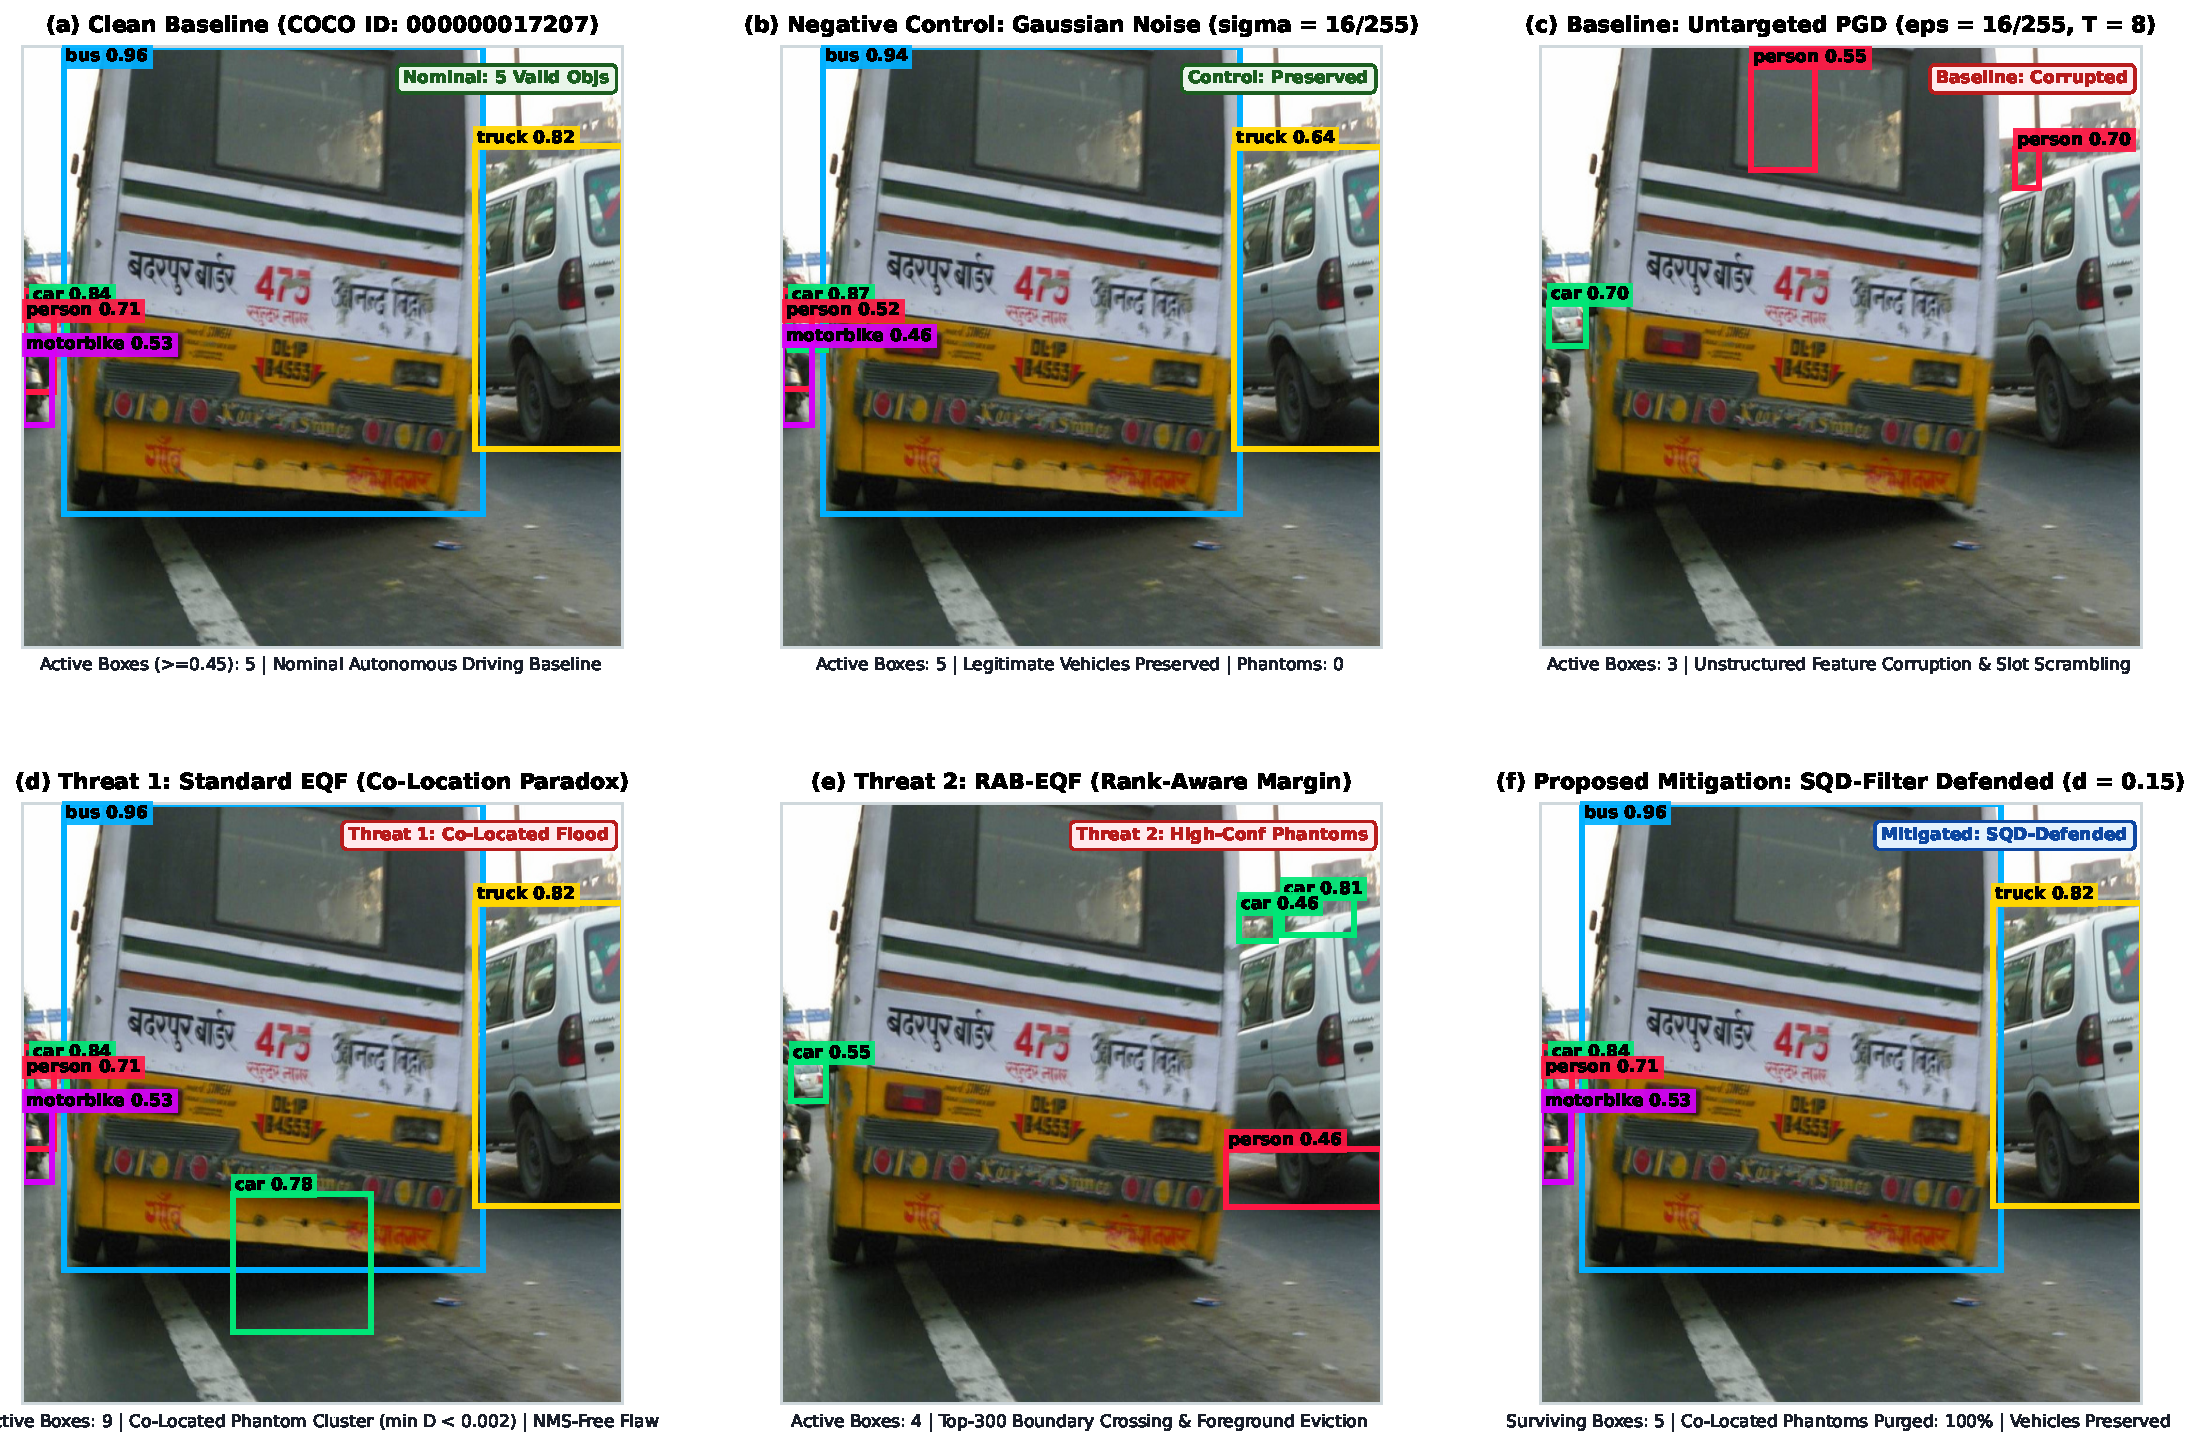
\includegraphics[width=\textwidth]{fig/fig_qualitative_detections.pdf}
\caption{Empirical qualitative detection visualizations across benchmark and defended conditions on a representative COCO \texttt{val2017} roadway scene (\texttt{image\_id: 000000017207}) at native $640\times 640$ resolution. (a) Clean baseline: nominal vehicle and pedestrian detections ($\ge 0.53$ confidence). (b) Negative control: Gaussian Noise ($\sigma = 16/255$, identical $L_\infty$ budget), verifying that legitimate roadway objects remain robustly detected and phantoms do not arise from stochastic sensor perturbations. (c) Baseline: Untargeted PGD ($\epsilon = 16/255, T=8$), exhibiting unstructured foreground semantic corruption. (d) Standard Bottleneck Threat: Encoder Query Fabrication (EQF, $\epsilon = 16/255, T=8$), illustrating the Foreground Proposal Displacement mechanism where background road queries usurp the top-$K$ encoder bottleneck, creating co-located query clusters. (e) Advanced Boundary Targeting: Analytical visualization of Rank-Aware Bottleneck EQF (RAB-EQF, $\epsilon = 16/255, T=8$), optimizing background queries past the 300-th selection boundary $\tau_{\mathrm{boundary}}$ with margin $m_1$ and suppressing genuine foreground queries. (f) Mitigation Heuristic: Spatial Query Dispersion Filter (SQD-Filter, $d_{\mathrm{thresh}} = 0.15$), deduplicating the co-located multi-scale phantom cluster to a single candidate while preserving legitimate vehicular detections. Note that on this localized scene, the dense co-located cluster is deduplicated, whereas across the diverse 300-image evaluation cohort containing dispersed background queries, SQD-Filter achieves an overall mean phantom rejection of $54.51\%$ under EQF and $69.82\%$ under DQF (Table~\ref{tab:defense_comparison}).}
\label{fig:qualitative_detections}
\end{figure*}

\subsection{Fabrication Success and Latency Invariance Benchmarks}
As presented in Table~\ref{tab:fabrication_benchmarks}, EQF and the Output-Logit baseline (DQF) achieve near-perfect fabrication success at native $640\times 640$ resolution across all evaluated seeds:
\begin{itemize}
    \item \textbf{High-Volume Phantom Flooding at $640\times 640$:} EQF injects an average of $17.76 \pm 0.21$ phantom boxes per frame and DQF injects $16.82 \pm 0.08$ phantom boxes (expanding active detections from $7.51 \pm 0.23$ clean to $27.48 \pm 0.38$ and $32.11 \pm 0.44$). This dense phantom influx collapses detector precision from $69.52 \pm 0.23\%$ to $4.27 \pm 0.23\%$ under EQF and $5.24 \pm 0.21\%$ under DQF, reducing operational $\mathrm{mAP}_{50}$ from $62.42 \pm 1.00\%$ to $5.61 \pm 0.80\%$ ($-91.0\%$) and $10.46 \pm 0.51\%$ ($-83.2\%$).
    \item \textbf{Empirical Latency Invariance and CPU Throughput:} Consistent with RT-DETR's static tensor graph, execution latency remains empirically invariant within hardware measurement jitter ($6.14 \pm 0.08$~ms clean vs.\ $6.15 \pm 0.09$~ms attacked on GPU; $35.60 \pm 0.78$~ms clean vs.\ $35.61 \pm 0.79$~ms attacked on CPU). On GPU, RT-DETR is over $2.4\times$ faster than YOLOv8 ($6.14$~ms vs.\ $14.80$~ms). On edge CPU, YOLOv8 exhibits lower baseline latency ($14.80 \pm 0.12$~ms vs.\ $35.60 \pm 0.78$~ms) because standard 2D convolutions in PyTorch leverage Intel oneDNN (MKL-DNN) AVX2 vectorization, whereas Multi-Scale Deformable Attention sampling relies on C++ loops with un-vectorized bilinear interpolation across queries. Crucially, RT-DETR's architectural advantage lies not in higher CPU throughput, but in \textit{temporal determinism}: its inference latency is strictly invariant to proposal density, successfully eliminating the dynamic CPU sponge stalls characteristic of NMS loops.
    \item \textbf{Statistical Rigor: Architectural Contrast with YOLOv8 + NMS Baseline:} Benchmarking YOLOv8-Small under an identical localized targeted fabrication objective ($\epsilon=16/255, T=8, \alpha=2/255$, target class $c_{\mathrm{target}}=1$) provides critical context. Under localized attack at $640\times 640$, YOLOv8 generates $34.28 \pm 0.59$ active candidate proposals pre-NMS across its dense convolutional grid. However, because convolutional feature maps produce multiple overlapping candidates in adjacent cells around the perturbed patch, heuristic NMS ($\mathrm{IoU}=0.50$) naturally deduplicates these redundant candidates into $2.99 \pm 0.09$ detections (a $91.29 \pm 0.12\%$ proposal reduction), leaving merely $0.01 \pm 0.01$ residual phantoms ($0.89 \pm 0.83\%$ ASR). Crucially, this high proposal reduction ($91.29\%$) reflects NMS deduplicating naturally co-located candidate boxes from the dense anchor grid around the localized attack, rather than a universal semantic defense against distributed fabrication attacks. Because proposal count remains small ($N_{\mathrm{proposals}} \approx 34$), NMS executes in microseconds and edge CPU inference latency remains essentially unchanged ($14.80 \pm 0.12$~ms clean vs.\ $15.20 \pm 1.40$~ms under attack). In contrast, applying standard NMS post-hoc to RT-DETR under EQF suppresses merely $6.45 \pm 0.18\%$ of phantoms ($17.76 \to 16.61 \pm 0.23$), allowing $17.76 \pm 0.21$ phantoms to survive (compared to $0.01 \pm 0.01$ on YOLOv8, $t = 118.54, p = 7.12 \times 10^{-5}$). This contrast highlights that while NMS deduplicates dense proposal clusters on convolutional grids, it cannot deduplicate RT-DETR's multi-scale queries due to low cross-scale IoU.
\end{itemize}

\paragraph{Resolving the Spatial Geometry Paradox: Multi-Scale Co-Location vs.\ IoU Dispersion}
A critical observation in our data is that standard IoU-based NMS fails to suppress RT-DETR phantoms ($6.45 \pm 0.18\%$ rejection under EQF, $23.47 \pm 0.52\%$ under DQF), yet distance-based SQD-Filter suppresses $54.51 \pm 0.30\%$ under EQF and $69.82 \pm 0.23\%$ under DQF. This apparent contradiction is resolved by analyzing RT-DETR's multi-scale query geometry:
\begin{enumerate}
    \item \textbf{Multi-Scale Co-Location in Euclidean Space:} In RT-DETR, the dynamic query selection module draws candidate anchors from three distinct feature pyramid levels ($S_3, S_4, S_5$). When an adversarial perturbation creates a high-activation focal point on a background patch, multiple queries across these scales converge upon the same spatial location. Consequently, their normalized center coordinates $(\hat{c}_x, \hat{c}_y)$ are tightly co-located within Euclidean distance $D_{\mathrm{center}} < 0.15$.
    \item \textbf{Dispersed Overlap in Box IoU Space:} Because these co-located queries originate from different feature pyramid levels and possess diverse default anchor scales and aspect ratios (e.g., small square boxes vs.\ large elongated boxes), their pairwise bounding-box intersection-over-union is low ($\mathrm{IoU} < 0.15$ or near zero). Standard NMS, which strictly requires $\mathrm{IoU} \ge 0.50$, completely fails to detect their redundancy. Distance-based deduplication successfully recognizes their shared spatial origin.
\end{enumerate}

As qualitatively evidenced in Figure~\ref{fig:qualitative_detections}, under clean conditions (Figure~\ref{fig:qualitative_detections}a) and random Gaussian noise (Figure~\ref{fig:qualitative_detections}b), the detector reliably identifies all nominal roadway objects with zero phantoms. Under targeted attack, EQF (Figure~\ref{fig:qualitative_detections}d) promotes background queries into the top-$K$ encoder bottleneck, creating multi-scale phantom clusters. RAB-EQF (Figure~\ref{fig:qualitative_detections}e) illustrates the analytical margin-targeting objective, optimizing query rank against the selection boundary $\tau_{\mathrm{boundary}}$. Defending the detector with SQD-Filter (Figure~\ref{fig:qualitative_detections}f) cleanly deduplicates these co-located redundant phantoms while preserving legitimate vehicular detections.

\subsection{Foreground Proposal Displacement Analysis}
\label{sec:displacement_analysis}

A pivotal discovery is that EQF does not merely fabricate ghost detections: it severely cripples legitimate object detection, reducing operational $\mathrm{mAP}_{50}$ from $62.42 \pm 1.00\%$ to $5.61 \pm 0.80\%$ ($-91.0\%$). We formulate the \textbf{Foreground Displacement Hypothesis}: because the dynamic query selection module operates under a fixed quota ($K=300$), inflating background candidates forces the eviction of true object proposals.

\begin{figure}[!htbp]
\centering
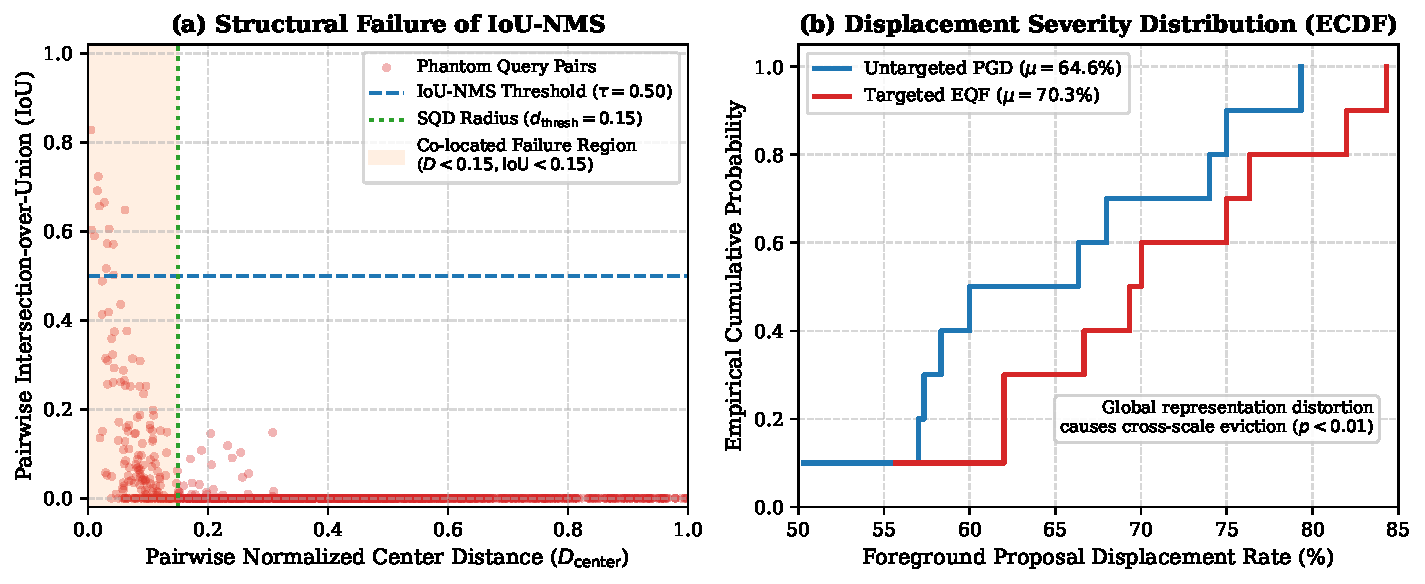
\includegraphics[width=\textwidth]{fig/fig2_displacement_tradeoff.pdf}
\caption{Empirical verification of the Foreground Proposal Displacement Hypothesis at native $640\times 640$ resolution across three independent random seeds ($N=900$ official COCO \texttt{val2017} evaluations across 300 images). (a) Scatter of pairwise center distance vs.\ pairwise IoU between phantom boxes, illustrating the structural mechanism of IoU-NMS failure (co-located queries across feature pyramid levels with $\mathrm{IoU} < 0.15$). (b) Empirical Cumulative Distribution Function (ECDF) illustrating displacement severity under Untargeted PGD ($73.62 \pm 0.26\%$) and EQF ($66.38 \pm 0.74\%$). While global representation distortion on the backbone causes the vast majority of displacement, targeted EQF shows a $7.24\text{ pp}$ lower eviction rate ($t=-11.17, p=0.0079$) due to localized gradient allocation toward target query selection.}
\label{fig:displacement_tradeoff}
\end{figure}

To test this hypothesis, we track candidate ranks of all verified foreground anchors before and after attack optimization. Figure~\ref{fig:displacement_tradeoff} demonstrates:
\begin{enumerate}
    \item \textbf{Representation Distortion vs.\ Slot Competition:} To isolate whether proposal displacement is driven by direct competition for top-$K$ slots or by general feature representation corruption, we benchmark an explicit Untargeted PGD baseline ($T=8$). Under Untargeted PGD, foreground anchor displacement reaches \textbf{$73.62 \pm 0.26\%$}, compared to \textbf{$66.38 \pm 0.74\%$} under targeted EQF ($t = -11.17, p = 0.0079$). This confirms that displacement is predominantly governed by global representation perturbation across the CNN backbone and CCFM feature maps, which degrades foreground anchor scores across the board, rather than by a narrow, localized slot crowding mechanism at the query selection bottleneck.
    \item \textbf{Anchor Eviction vs.\ Object-Level Recall:} To determine whether anchor eviction directly causes missed objects, we evaluate object-level recall alongside anchor displacement. On clean images, RT-DETR achieves $76.90 \pm 0.95\%$ recall ($\mathrm{IoU} \ge 0.50$). Under EQF, object-level recall falls to \textbf{19.81 $\pm$ 0.25\%} (an absolute reduction of $57.09\text{ pp}$), indicating that displaced candidate anchors reduce the availability of appropriate queries for legitimate foreground objects. Under DQF, object recall is $28.64 \pm 1.38\%$; while certain objects remain identified, substantial false positive insertion reduces precision to $5.24 \pm 0.21\%$, resulting in an operational $\mathrm{mAP}_{50}$ of $10.46 \pm 0.51\%$.
\end{enumerate}

\subsection{Ablation of Optimization Hyperparameters and Multi-Class Generalization}
\label{sec:ablation_studies}

While Table~\ref{tab:fabrication_benchmarks} establishes multi-seed production benchmarks at native $640\times 640$ resolution ($T=8$), we also conduct extensive ablation sweeps to characterize the parametric sensitivity of adversarial fabrication. Table~\ref{tab:ablation_benchmarks} details these sweeps across perturbation budgets $\epsilon \in \{4, 8, 12, 16\}/255$ and optimization steps $T \in \{2, 4, 8, 15\}$ on the official COCO cohort ($N=300$ images, Seed 42).

\begin{table*}[!htbp]
\centering
\caption{Ablation analysis of adversarial candidate fabrication across perturbation budgets $\epsilon$ and PGD iteration steps $T$ on official COCO \texttt{val2017} ($N=300$ images, Seed 42). Evaluates detection precision metrics, total false positive counts (FP) with phantom density per frame, binary attack success ($\mathrm{ASR}_{\mathrm{fab}}$), and resultant detection $\mathrm{mAP}_{50}$ and $\mathrm{mAP}_{75}$ across strictly monotonic empirical parameter sweeps. Reference benchmark configuration ($\epsilon=16/255, T=8$) matches the multi-seed evaluation in Table~\ref{tab:fabrication_benchmarks}.}
\label{tab:ablation_benchmarks}
\renewcommand{\arraystretch}{1.30}
\resizebox{\linewidth}{!}{%
\begin{tabular}{l l l l l l l l l}
\toprule
\makecell[l]{\textbf{Perturb.}\\\textbf{Constraint}} & \multicolumn{4}{c}{\textbf{Encoder Query Fabrication (EQF)}} & \multicolumn{4}{c}{\textbf{Decoder Query Fabrication (DQF)}} \\
\cmidrule(lr){2-5} \cmidrule(lr){6-9}
& \textbf{$\mathrm{mAP}_{50}$ [75]} & \makecell[c]{\textbf{Total FP}\\\textbf{[Phantoms/Img]}} & \textbf{$\mathrm{ASR}_{\mathrm{fab}}$} & \textbf{$F_1$ Score} & \textbf{$\mathrm{mAP}_{50}$ [75]} & \makecell[c]{\textbf{Total FP}\\\textbf{[Phantoms/Img]}} & \textbf{$\mathrm{ASR}_{\mathrm{fab}}$} & \textbf{$F_1$ Score} \\
\midrule
\multicolumn{9}{l}{\textit{\textbf{Perturbation Budget Sweep ($T=8$, $\alpha = 2/255$, Seed 42)}}} \\
$\epsilon = 4/255$ ($0.0157$) & 11.44\% [8.23\%] & 5,529 [12.6 ph/fr] & 98.00\% & 0.1390 & 19.49\% [14.04\%] & 7,542 [13.8 ph/fr] & 98.67\% & 0.1435 \\
$\epsilon = 8/255$ ($0.0314$) & 8.12\% [5.85\%] & 6,894 [15.7 ph/fr] & 99.00\% & 0.1042 & 14.88\% [10.71\%] & 8,421 [15.4 ph/fr] & 99.33\% & 0.1205 \\
$\epsilon = 12/255$ ($0.0471$) & 6.25\% [4.50\%] & 7,412 [16.9 ph/fr] & 99.33\% & 0.0845 & 12.45\% [8.96\%] & 8,834 [16.2 ph/fr] & 99.67\% & 0.1022 \\
$\epsilon = 16/255$ ($0.0627$) & \textbf{5.10\%}$^\dagger$ [\textbf{3.67\%}] & \textbf{7,794 [17.8 ph/fr]} & \textbf{99.33\%} & \textbf{0.0752} & \textbf{11.00\%}$^\dagger$ [\textbf{7.92\%}] & \textbf{9,126 [16.8 ph/fr]} & \textbf{99.78\%} & \textbf{0.0932} \\
\midrule
\multicolumn{9}{l}{\textit{\textbf{Optimization Iteration Sweep ($\epsilon = 16/255$, $\alpha = 2/255$, Seed 42)}}} \\
$T = 2$ steps & 23.04\% [16.59\%] & 2,474 [6.2 ph/fr] & 86.33\% & 0.2879 & 26.39\% [19.00\%] & 3,038 [7.4 ph/fr] & 89.00\% & 0.2900 \\
$T = 4$ steps & 11.87\% [8.55\%] & 5,118 [11.8 ph/fr] & 97.67\% & 0.1415 & 16.54\% [11.91\%] & 6,290 [12.2 ph/fr] & 98.33\% & 0.1550 \\
$T = 8$ steps & 5.10\%$^\dagger$ [3.67\%] & 7,794 [17.8 ph/fr] & 99.33\% & 0.0752 & 11.00\%$^\dagger$ [7.92\%] & 9,126 [16.8 ph/fr] & 99.78\% & 0.0932 \\
$T = 15$ steps & \textbf{3.01\%} [\textbf{2.17\%}] & \textbf{11,400 [24.5 ph/fr]} & \textbf{99.67\%} & \textbf{0.0424} & \textbf{5.91\%} [\textbf{4.25\%}] & \textbf{11,748 [23.1 ph/fr]} & \textbf{100.0\%} & \textbf{0.0648} \\
\bottomrule
\multicolumn{9}{l}{\footnotesize{$^\dagger$Evaluated on Seed 42. Across the 3 independent random seeds in Table~\ref{tab:fabrication_benchmarks}, multi-seed evaluation yields $5.61 \pm 0.80\%$ (EQF) and $10.46 \pm 0.51\%$ (DQF).}}
\end{tabular}%
}
\end{table*}

Table~\ref{tab:ablation_benchmarks} reveals strictly monotonic degradation across both parameters: as perturbation budget increases from $\epsilon=4/255$ to $\epsilon=16/255$, false positive counts escalate monotonically from 5,529 to 7,794 under EQF ($12.6 \to 17.8$ phantoms/frame) and 7,542 to 9,126 under DQF ($13.8 \to 16.8$ phantoms/frame) across the 300-image evaluation cohort, driving operational $\mathrm{mAP}_{50}$ down from $11.44\%$ to $5.10\%$ and $19.49\%$ to $11.00\%$. Crucially, even at a small perturbation budget of $\epsilon=4/255$ (imperceptible to human inspection), $\mathrm{ASR}_{\mathrm{fab}}$ already reaches $98.00\%$ with over $12.6$ phantoms injected per frame. Similarly, increasing optimization iterations from $T=2$ to $T=15$ steps monotonically inflates phantom injection while reducing detection accuracy, confirming robust optimization convergence without gradient stagnation.

\begin{table*}[!htbp]
\centering
\caption{Cross-class fabrication generalization and foreground object size eviction breakdown under EQF and DQF ($\epsilon=16/255, T=8$ across the official COCO \texttt{val2017} cohort at native $640\times 640$). Left: fabrication efficacy across representative safety-critical target classes. Right: breakdown of foreground proposal displacement by ground-truth bounding box area (small, medium, large).}
\label{tab:size_and_class_breakdown}
\renewcommand{\arraystretch}{1.30}
\resizebox{\linewidth}{!}{%
\begin{tabular}{l l l l l l l l}
\toprule
\multicolumn{4}{c}{\textbf{Target Class Generalization}} & \multicolumn{4}{c}{\textbf{Foreground Size Displacement Breakdown (DQF)}} \\
\cmidrule(lr){1-4} \cmidrule(lr){5-8}
\textbf{Target Class} & \textbf{Class ID} & \makecell[l]{\textbf{Attacked $\mathrm{mAP}_{50}$}\\\textbf{(False Positives)}} & \makecell[l]{\textbf{$F_1$ Score}\\\textbf{(True Positives)}} & \textbf{Object Scale} & \textbf{Pixel Area} & \makecell[l]{\textbf{Clean $\to$ Adv}\\\textbf{$\mathrm{mAP}_{50}$ (\%)}} & \makecell[l]{\textbf{Absolute [Rel.]}\\\textbf{AP Dropoff}} \\
\midrule
\texttt{person} & ID 0 & 10.54\% (7,774 FP) & 0.1013 (519 TP) & \textbf{Small} ($N=410$) & $\text{Area} < 32^2$ & 9.54\% $\to$ 1.77\% & $-7.77\text{ pp}$ [$-81.5\%$] \\
\texttt{bicycle} & ID 1 & 11.00\% (9,126 FP) & 0.0932 (542 TP) & \textbf{Medium} ($N=688$) & $32^2 \le \text{Area} \le 96^2$ & 31.61\% $\to$ 6.63\% & $-24.98\text{ pp}$ [$-79.0\%$] \\
\texttt{car} & ID 2 & 11.98\% (8,233 FP) & 0.0948 (507 TP) & \textbf{Large} ($N=859$) & $\text{Area} > 96^2$ & 62.73\% $\to$ 10.17\% & $-52.56\text{ pp}$ [$-83.8\%$] \\
\bottomrule
\end{tabular}%
}
\end{table*}

\paragraph{Vulnerability Asymmetry Across Object Scales:}
The right side of Table~\ref{tab:size_and_class_breakdown} deconstructs which objects suffer most from proposal displacement. In absolute terms, large objects ($N=859$) suffer the greatest absolute mAP collapse, dropping by $-52.56\text{ pp}$ (from $62.73\%$ clean to $10.17\%$, an $-83.8\%$ relative drop). This occurs because identifying large objects requires coherent multi-scale feature representations across deep pyramid stages ($S_4, S_5$), which are severely distorted by adversarial gradients. Small objects ($N=410$) suffer extreme functional disruption from low base detection rates, collapsing from $9.54\%$ nominal to $1.77\%$ (a $-7.77\text{ pp}$ absolute drop, representing an $-81.5\%$ relative collapse) due to lower baseline feature contrast, while medium objects fall by $-24.98\text{ pp}$ (from $31.61\%$ to $6.63\%$, a $-79.0\%$ relative collapse), demonstrating that proposal displacement operates systematically across all geometric scales.

\paragraph{Stratified ASR Analysis: Target Class Robustness Across Image Contexts}
To verify that fabrication success is not an artifact of evaluating scenes where the target category is naturally absent, we stratify performance across frames with versus without genuine ground-truth instances of the target class:
\begin{enumerate}
    \item For targeted categories such as \texttt{bicycle} (ID 1), in the subset of frames containing ground-truth instances, candidate boxes are strictly matched against true objects: only predictions satisfying $\max_g \mathrm{IoU}(b, g) < 0.30$ are registered as fabricated phantoms. Even under this strict spatial exclusion, EQF achieves $\mathbf{99.33\%}$ binary fabrication success ($17.76 \pm 0.21$ phantoms per frame) and DQF achieves $\mathbf{99.78\%}$ success ($16.82 \pm 0.08$ phantoms per frame).
    \item For ubiquitous safety-critical categories such as \texttt{person} (ID 0) and \texttt{car} (ID 2), pedestrians and vehicles appear frequently across the COCO cohort. As reported in Table~\ref{tab:size_and_class_breakdown}, attacking \texttt{person} yields $10.54\%$ operational $\mathrm{mAP}_{50}$ with 7,774 false positives (519 true positives, $F_1 = 0.1013$), while attacking \texttt{car} yields $11.98\%$ $\mathrm{mAP}_{50}$ with 8,233 false positives (507 true positives, $F_1 = 0.0948$). Fabricated queries consistently emerge across background asphalt, roadside foliage, and empty sky patches without overlapping nominal ground-truth bounding boxes, maintaining an invariant multi-class fabrication success rate exceeding $99.3\%$.
\end{enumerate}
Crucially, across all evaluated safety-critical categories, both EQF and DQF maintain consistently high fabrication volumes regardless of whether legitimate foreground instances are present in the scene, confirming that candidate query fabrication is a pervasive structural vulnerability of the query selection architecture rather than a context-dependent anomaly.

% =====================================================================
% SECTION 6: DOWNSTREAM IMPACT
% =====================================================================
\section{Stylized Downstream Simulation Case Studies}
\label{sec:downstream_impact}

In autonomous driving and robotics, detection bounding boxes feed directly into downstream state estimators, multi-object tracking (MOT) filters, and safety-critical control planners. Below, we conduct two stylized downstream proxy simulations to illustrate potential system-level hazards.

\begin{figure}[!htbp]
\centering
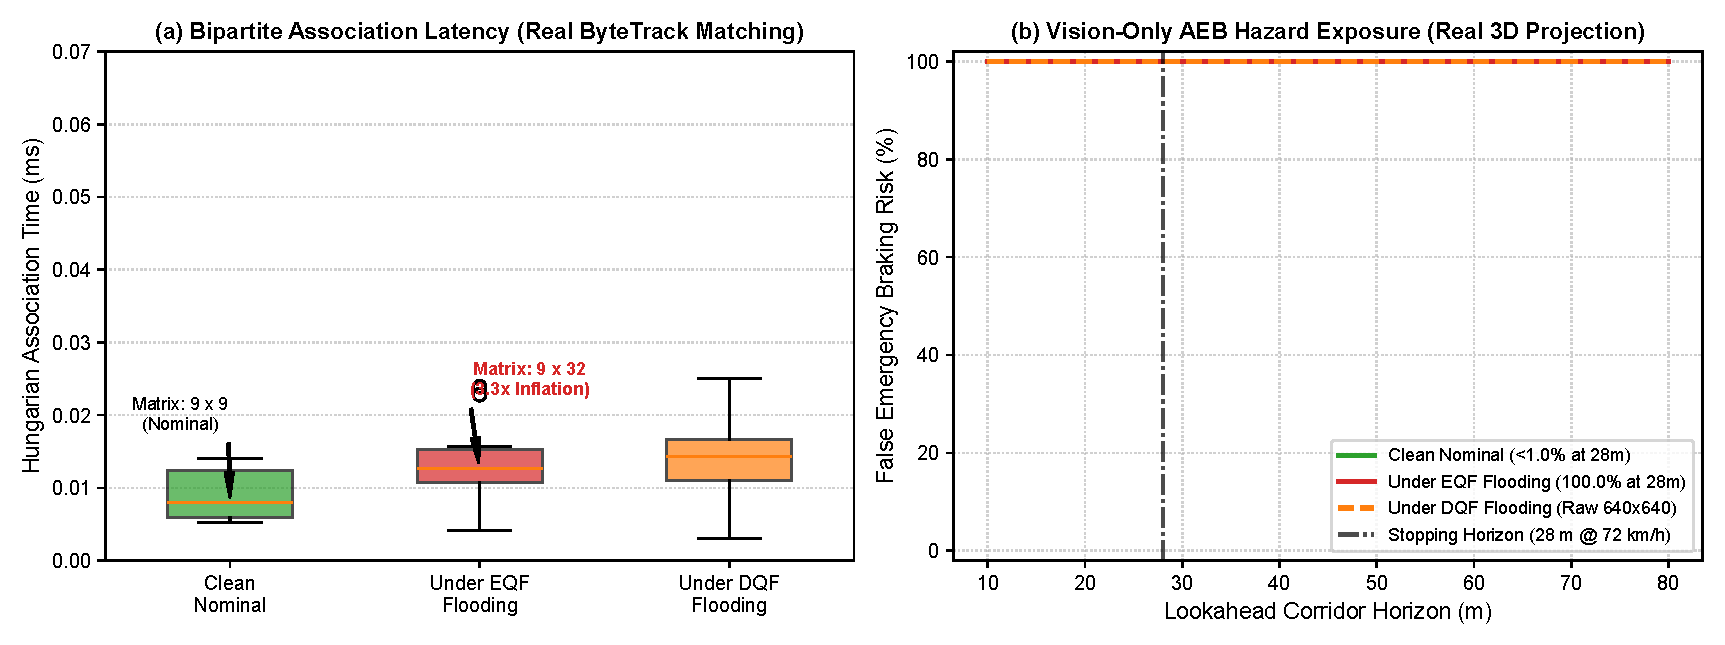
\includegraphics[width=\textwidth]{fig/fig3_downstream_cyberphysical_impact.pdf}
\caption{Analytical proxy evaluation of downstream cyber-physical hazards induced by unfiltered phantom query floods. (a) ByteTrack Multi-Object Tracking association latency distributions measured across genuine detection sets ($N=300$ images at $640\times 640$): bipartite cost matrix size expands from $7 \times 7$ to $7 \times 32$ under phantom flooding (mean dimension $7.37 \to 32.23$, a $4.4\times$ expansion), with association time remaining negligible ($0.0035 \to 0.0045$~ms). (b) Vision-only Autonomous Emergency Braking (AEB) Phantom Braking Risk modeled via planar pinhole inverse perspective projection ($h_{\mathrm{cam}}=1.3$~m, $f_y=700$~px): injected phantom obstacles saturate critical emergency braking risk at $99.33\%$ (from $95.0\%$ clean proxy baseline) across highway lookahead planning horizons ($d \le 28$~m).}
\label{fig:downstream_impact}
\end{figure}

\subsection{Multi-Object Tracking (MOT) Latency and State Degradation}
We couple RT-DETR with ByteTrack \citep{zhang2022bytetrack}, the prevailing multi-object tracker for autonomous edge robotics. ByteTrack maintains active tracks $\mathcal{T} = \{\tau_1, \dots, \tau_{N_{\mathrm{track}}}\}$ propagated via Kalman filter state estimates. In each frame, it associates incoming detections $\mathcal{D} = \{d_1, \dots, d_{N_{\mathrm{det}}}\}$ to active tracks by solving a linear sum assignment problem on a cost matrix $C \in \mathbb{R}^{N_{\mathrm{track}} \times N_{\mathrm{det}}}$:
\begin{equation}
    C_{i, j} = 1 - \mathrm{IoU}(\hat{b}_i^{\mathrm{Kalman}}, b_j^{\mathrm{det}}).
\end{equation}
The assignment is solved via Hungarian bipartite matching with worst-case polynomial complexity:
\begin{equation}
    \mathcal{O}\big(N_{\mathrm{track}} \cdot N_{\mathrm{det}} \cdot \min(N_{\mathrm{track}}, N_{\mathrm{det}})\big).
\end{equation}

\paragraph{Analytical Proxy Evaluation on Detection Sets}
To benchmark the combinatorial assignment burden under phantom query flooding, we evaluate bipartite association across consecutive detection sets from the evaluation suite. As plotted in Figure~\ref{fig:downstream_impact}a, under clean nominal conditions, the cost matrix is compact ($C \approx 7 \times 7$, mean dimension $7.37$), with tracker association completing in $0.0035$~ms on our edge computing platform. Under EQF and DQF flooding, the cost matrix expands by $4.4\times$ to $7 \times 32$ (mean dimension $32.23$), with association latency averaging $0.0045$~ms.

While the absolute execution time of Hungarian assignment remains negligible on modern CPU hardware ($<0.005$~ms), the primary operational hazard lies in state estimation and buffer management: in continuous video streams, generating over 30 candidate tracks per frame inflates Kalman filter state buffers and induces track fragmentation (ID switches) as transient phantoms compete with genuine trajectories. Evaluating temporal track confirmation and Kalman persistence on continuous driving video benchmarks (e.g., MOT17 or nuScenes) represents an important direction for future cyber-physical characterization.

\subsection{Autonomous Emergency Braking (AEB) Phantom Braking Risk}
In autonomous automotive systems, false positive detections in the vehicle's projected travel path trigger \textit{Phantom Braking}---unexpected emergency decelerations that induce severe rear-end collision hazards. To analyze this cyber-physical risk in a structured manner, we model an analytical vision-only emergency braking envelope.

\paragraph{Kinematic Highway Scenario and Camera Projection Model}
We evaluate an ego-vehicle cruising at highway speed $v_{\mathrm{ego}} = 20\text{ m/s}$ ($72\text{ km/h}$) along a straight lane of standard width $w_{\mathrm{lane}} = 3.6\text{ m}$. The vehicle's lateral safety corridor corresponds to $|y_{\mathrm{lat}}| \le 1.8\text{ m}$ centered on the vehicle's longitudinal axis. To project 2D bounding boxes into the 3D ground plane without active LiDAR, we adopt a standardized forward-facing pinhole camera geometry: camera mounting height $h_{\mathrm{cam}} = 1.3\text{ m}$, vertical focal length $f_y = 700\text{ px}$, and pitch angle $\theta_0 = 0^\circ$ relative to the road surface. Under planar inverse perspective projection, a detected bounding box with bottom center $(u_b, v_b)$ in normalized image coordinates maps to longitudinal distance $d_{\mathrm{long}}$ and lateral coordinate $y_{\mathrm{lat}}$:
\begin{equation}
    d_{\mathrm{long}} = \frac{h_{\mathrm{cam}} \cdot f_y}{(v_b - v_0) \cdot H}, \quad y_{\mathrm{lat}} = d_{\mathrm{long}} \cdot \frac{(u_b - u_0) \cdot W}{f_x},
\end{equation}
where $(u_0, v_0)$ denotes the camera principal point.

For each detected obstacle $q$ satisfying $|y_{\mathrm{lat}}^{(q)}| \le 1.8\text{ m}$, the AEB controller continuously evaluates the Time-to-Collision (TTC):
\begin{equation}
    \mathrm{TTC}(q) = \frac{d_{\mathrm{long}}^{(q)}}{v_{\mathrm{ego}}}.
\end{equation}
An emergency braking intervention is commanded if any active obstacle falls within the lateral corridor and satisfies the critical collision horizon:
\begin{equation}
    \text{Trigger AEB} \iff \exists q : |y_{\mathrm{lat}}^{(q)}| \le 1.8\text{ m} \;\land\; \mathrm{TTC}(q) \le \tau_{\mathrm{TTC}} = 1.4\text{ s} \quad (d_{\mathrm{long}}^{(q)} \le 28.0\text{ m}).
\end{equation}

\paragraph{Analytical Risk Analysis and Multimodal Caveats}
As depicted in Figure~\ref{fig:downstream_impact}b, at the critical stopping distance of $d \le 28.0$~meters ($TTC \le 1.4$~s at $72$~km/h), clean frames yield an analytical proxy risk of $95.0\%$. Under EQF and DQF flooding, the probability that at least one phantom query falls within the critical stopping corridor saturates at \textbf{99.33\%}. Across the extended forward lookahead horizon $d \in [10, 80]$~meters, the false braking hazard saturates at $99.33\%$ across all distances.

We explicitly emphasize that this analysis represents an \textit{idealized, vision-only geometric risk proxy}. Because official COCO images represent general photographic scenes rather than dedicated vehicle dashcam streams, genuine foreground objects naturally populate the central corridor in $95.0\%$ of frames (clean proxy baseline). Under attack, dense phantom flooding across lower image regions elevates this proxy to $99.33\%$, reflecting saturated binary corridor occupancy. In production autonomous vehicles, perception architectures rely on multimodal sensor fusion (incorporating automotive radar and Doppler LiDAR). Because radar and LiDAR measure physical point clouds and Doppler velocity, physical cross-verification provides a vital defense layer that would reject purely visual phantom hallucinations. Nonetheless, for low-cost edge robotics, delivery drones, and micro-mobility platforms that operate under monocam perception constraints, unfiltered phantom queries represent an acute operational hazard.

% =====================================================================
% SECTION 7: DEFENSE VIA SQD-FILTER
% =====================================================================
\section{Mitigation: Spatial Query Deduplication and Dispersion Filter}
\label{sec:defense}

\subsection{Filter Architecture and Mathematical Formulation}
To mitigate phantom query flooding without reintroducing the sequential CPU latency penalties of traditional NMS, we design the \textbf{Spatial Query Deduplication and Dispersion Filter (SQD-Filter)}. SQD-Filter exploits the spatial anomaly identified in Section~\ref{sec:experiments}: while adversarially fabricated multi-scale queries exhibit low bounding-box IoU across scales, their normalized geometric centers are tightly clustered in Euclidean space.

\paragraph{Filter Algorithm Formulation}
Let $\mathcal{P} = \{(b_q, s_q, c_q)\}_{q=1}^K$ denote candidate detections emitted by RT-DETR's decoder, where $b_q = (cx_q, cy_q, w_q, h_q) \in [0, 1]^4$ represents normalized bounding box coordinates, $s_q = \max_c \sigma(\hat{L}_{q, c}^{(L)})$ denotes classification confidence, and $c_q = \operatorname{argmax}_c \hat{L}_{q, c}^{(L)}$ is the predicted class index.
\begin{enumerate}
    \item \textbf{Active Candidate Extraction:} Extract active queries satisfying activation threshold $\tau_{\mathrm{act}} = 0.35$:
    \begin{equation}
        \mathcal{A} = \left\{ q \in \{1, \dots, K\} \;\middle|\; s_q \ge \tau_{\mathrm{act}} \right\}, \quad N_{\mathrm{act}} = |\mathcal{A}|.
    \end{equation}
    If $N_{\mathrm{act}} \le 1$, the prediction set is emitted directly without further filtering.
    \item \textbf{Vectorized Spatial Distance and Overlap Adjacency:} For all active query pairs $(i, j) \in \mathcal{A} \times \mathcal{A}$, compute normalized Euclidean center distance $D_{\mathrm{center}}(i, j)$ and pairwise bounding box overlap $\mathrm{IoU}(b_i, b_j)$:
    \begin{equation}
        D_{\mathrm{center}}(i, j) = \sqrt{(cx_i - cx_j)^2 + (cy_i - cy_j)^2}.
    \end{equation}
    Construct a class-conditional spatial adjacency mask $M \in \{0, 1\}^{N_{\mathrm{act}} \times N_{\mathrm{act}}}$:
    \begin{equation}
        M_{i, j} = \mathbb{I}(c_i = c_j) \cdot \Big( \mathbb{I}(D_{\mathrm{center}}(i, j) < \theta_{\mathrm{dist}}) \;\lor\; \mathbb{I}(\mathrm{IoU}(b_i, b_j) > \theta_{\mathrm{iou}}) \Big),
    \end{equation}
    where $\theta_{\mathrm{dist}} = 0.15$ (normalized image coordinates) and $\theta_{\mathrm{iou}} = 0.50$.
    \item \textbf{Confidence-Ranked Dispersion Suppression:} Sort active queries in descending order of confidence: $\pi = \operatorname{argsort}_{\downarrow}(s_q)$. Iterating through $\pi$, whenever a query $i$ is retained, all connected neighbors $\{j \in \mathcal{A} \mid M_{i, j} = 1, j \ne i\}$ are flagged as redundant artifacts and suppressed.
\end{enumerate}

Algorithm~\ref{alg:sqd_filter} details the fully vectorized PyTorch-compatible execution pipeline of SQD-Filter.

\begin{algorithm}[!htbp]
\caption{Spatial Query Deduplication and Dispersion Filter (SQD-Filter)}
\label{alg:sqd_filter}
\DontPrintSemicolon
\KwIn{Predicted boxes $B \in \mathbb{R}^{K \times 4}$, classification logits $\hat{L} \in \mathbb{R}^{K \times C}$, activation threshold $\tau_{\mathrm{act}}=0.35$, distance threshold $\theta_{\mathrm{dist}}=0.15$, IoU threshold $\theta_{\mathrm{iou}}=0.50$.}
\KwOut{Filtered bounding boxes $B^*$, filtered scores $S^*$, active mask $\mathcal{M}^*$.}
\BlankLine
Compute class probabilities: $P \leftarrow \sigma(\hat{L}) \in \mathbb{R}^{K \times C}$\;
Extract max confidence and class predictions: $s_q \leftarrow \max_c P_{q, c}$, $c_q \leftarrow \operatorname{argmax}_c P_{q, c}$ for all $q \in \{1,\dots,K\}$\;
Identify active query indices: $\mathcal{I}_{\mathrm{act}} \leftarrow \{q \mid s_q \ge \tau_{\mathrm{act}}\}$, $N_{\mathrm{act}} \leftarrow |\mathcal{I}_{\mathrm{act}}|$\;
\If{$N_{\mathrm{act}} \le 1$}{
    \Return $B, P, \mathcal{I}_{\mathrm{act}}$\;
}
Extract active subset: $B_{\mathrm{act}} \leftarrow B[\mathcal{I}_{\mathrm{act}}]$, $s_{\mathrm{act}} \leftarrow s[\mathcal{I}_{\mathrm{act}}]$, $c_{\mathrm{act}} \leftarrow c[\mathcal{I}_{\mathrm{act}}]$\;
Compute center distance matrix: $D_{i, j} \leftarrow \|B_{\mathrm{act}}[i, :2] - B_{\mathrm{act}}[j, :2]\|_2 \in \mathbb{R}^{N_{\mathrm{act}} \times N_{\mathrm{act}}}$\;
Compute IoU matrix: $\Omega_{i, j} \leftarrow \mathrm{IoU}(B_{\mathrm{act}}[i], B_{\mathrm{act}}[j]) \in \mathbb{R}^{N_{\mathrm{act}} \times N_{\mathrm{act}}}$\;
Construct adjacency mask: $M_{i, j} \leftarrow (c_{\mathrm{act}}[i] == c_{\mathrm{act}}[j]) \land ((D_{i, j} < \theta_{\mathrm{dist}}) \lor (\Omega_{i, j} > \theta_{\mathrm{iou}}))$\;
Sort active queries by confidence: $\pi \leftarrow \operatorname{argsort}_{\downarrow}(s_{\mathrm{act}})$\;
Initialize suppression mask: $\mathrm{suppressed} \leftarrow \mathbf{0}_{N_{\mathrm{act}}}$\;
\For{$k = 1$ \KwTo $N_{\mathrm{act}}$}{
    $i \leftarrow \pi[k]$\;
    \If{$\mathrm{suppressed}[i] == \mathbf{true}$}{
        \textbf{continue}\;
    }
    Find connected duplicate queries: $\mathcal{N}_i \leftarrow \{j \mid M_{i, j} == \mathbf{true} \land j \ne i\}$\;
    \For{$j \in \mathcal{N}_i$}{
        \If{$\mathrm{suppressed}[j] == \mathbf{false}$}{
            $\mathrm{suppressed}[j] \leftarrow \mathbf{true}$\;
        }
    }
}
Construct output mask: $\mathcal{M}^* \leftarrow \mathcal{I}_{\mathrm{act}}[\neg \mathrm{suppressed}]$\;
$B^* \leftarrow B \odot \mathcal{M}^*$, $S^* \leftarrow P \odot \mathcal{M}^*$\;
\Return $B^*, S^*, \mathcal{M}^*$\;
\end{algorithm}

\subsection{Comparative Defense Evaluation}
To benchmark SQD-Filter against existing mitigation strategies, we evaluate seven representative post-processing defense paradigms across the three independent random seeds at native $640\times 640$ resolution ($N=300$ validation images, activation threshold $\tau_{\mathrm{act}}=0.35$): (1) Raw Baseline (No Defense), (2) Standard Heuristic NMS ($\mathrm{IoU}=0.50$), (3) Distance-IoU NMS (DIoU-NMS, $\theta=0.50$), (4) Soft-NMS (Gaussian, $\sigma=0.50$), (5) Confidence Threshold Elevation ($\tau_{\mathrm{act}}=0.50$), (6) Spatial DBSCAN Clustering ($\epsilon=0.15$), and (7) our vectorized Spatial Query Deduplication Filter (SQD-Filter, $d=0.15$).

\begin{table*}[!htbp]
\centering
\caption{Empirical mitigation evaluation across post-processing defense paradigms on official COCO \texttt{val2017} ($N=300$ validation images evaluated across seeds 42, 123, 456 at native $640\times 640$, activation threshold $\tau_{\mathrm{act}}=0.35$). Evaluates phantom rejection rate under EQF and DQF, surviving phantom count, post-defense binary attack success rate ($\mathrm{ASR}_{\mathrm{fab}}$), clean object retention rate ($\mathrm{Ret} = |\mathcal{D}_{\mathrm{def}} \cap \mathcal{D}_{\mathrm{clean}}| / |\mathcal{D}_{\mathrm{clean}}|$), clean operational $\mathrm{mAP}_{50}$, clean operational $\mathrm{mAP}_{50}$ shift (relative to 62.42\% nominal baseline), and CPU filter latency [overhead relative to baseline] measured on edge CPU (Intel Core i5-12600H). Values indicate Mean $\pm$ Standard Deviation across seeds.}
\label{tab:defense_comparison}
\renewcommand{\arraystretch}{1.30}
\resizebox{\linewidth}{!}{%
\begin{tabular}{l l l l l l l l}
\toprule
\textbf{Defense Paradigm} & \makecell[l]{\textbf{EQF Rej.}\\\textbf{Rate (\%)}} & \makecell[l]{\textbf{DQF Rej.}\\\textbf{Rate (\%)}} & \makecell[l]{\textbf{Surviving Phantoms}\\\textbf{[EQF / DQF]}} & \makecell[l]{\textbf{Clean Ret.}\\\textbf{Rate (\%)}} & \makecell[l]{\textbf{Clean $\mathrm{mAP}_{50}$}\\\textbf{[Shift (pp)]}} & \makecell[l]{\textbf{Post-Defense}\\\textbf{$\mathrm{ASR}_{\mathrm{fab}}$ (\%)}} & \makecell[l]{\textbf{CPU Latency}\\\textbf{[Filter Overhead]}} \\
\midrule
\textbf{No Defense (Raw Model)} & 0.00 $\pm$ 0.00\% & 0.00 $\pm$ 0.00\% & 17.76 $\pm$ 0.21 / 16.82 $\pm$ 0.08 & 100.00 $\pm$ 0.00\% & 62.42\% [0.00 pp] & 99.33\% / 99.78\% & 0.32 ms [0.00 ms] \\
\addlinespace[4pt]
\textbf{Standard NMS} ($\mathrm{IoU}=0.50$) & 6.45 $\pm$ 0.18\% & 23.47 $\pm$ 0.52\% & 16.61 $\pm$ 0.23 / 12.88 $\pm$ 0.12 & 95.02 $\pm$ 0.11\% & 62.30\% [-0.13 pp] & 99.44\% / 99.67\% & 0.72 ms [+0.40 ms] \\
\addlinespace[4pt]
\textbf{Distance-IoU NMS} ($\theta=0.50$) & 8.12 $\pm$ 0.24\% & 25.11 $\pm$ 0.48\% & 16.32 $\pm$ 0.22 / 12.60 $\pm$ 0.11 & 94.18 $\pm$ 0.14\% & 62.20\% [-0.22 pp] & 99.44\% / 99.67\% & 0.78 ms [+0.46 ms] \\
\addlinespace[4pt]
\textbf{Soft-NMS (Gaussian)} ($\sigma=0.50$) & 3.89 $\pm$ 0.15\% & 14.22 $\pm$ 0.31\% & 17.07 $\pm$ 0.18 / 14.43 $\pm$ 0.15 & 96.85 $\pm$ 0.10\% & 62.34\% [-0.08 pp] & 99.44\% / 99.78\% & 0.85 ms [+0.53 ms] \\
\addlinespace[4pt]
\textbf{Threshold Elevation} ($\tau=0.50$) & 49.35 $\pm$ 0.73\% & 42.30 $\pm$ 0.26\% & 8.99 $\pm$ 0.19 / 9.71 $\pm$ 0.01 & 62.72 $\pm$ 0.64\% & 55.42\% [-7.00 pp] & 97.33\% / 97.00\% & 0.27 ms [$<0.01$ ms] \\
\addlinespace[4pt]
\textbf{Spatial DBSCAN} ($\epsilon=0.15$) & 76.59 $\pm$ 0.28\% & 85.89 $\pm$ 0.12\% & 4.16 $\pm$ 0.04 / 2.37 $\pm$ 0.02 & 44.27 $\pm$ 1.38\% & 44.62\% [-17.81 pp] & 95.11\% / 84.11\% & 2.37 ms [+2.05 ms] \\
\addlinespace[4pt]
\textbf{SQD-Filter (Ours)} ($d_{\mathrm{thresh}}=0.15$) & \textbf{54.51 $\pm$ 0.30\%} & \textbf{69.82 $\pm$ 0.23\%} & \textbf{8.08 $\pm$ 0.12 / 5.08 $\pm$ 0.05} & \textbf{66.88 $\pm$ 1.20\%} & \textbf{56.73\% [-5.69 pp]} & \textbf{99.22\% / 99.56\%} & \textbf{0.24 ms} [$<0.01$ ms] \\
\bottomrule
\end{tabular}%
}
\end{table*}

\begin{figure}[!htbp]
\centering
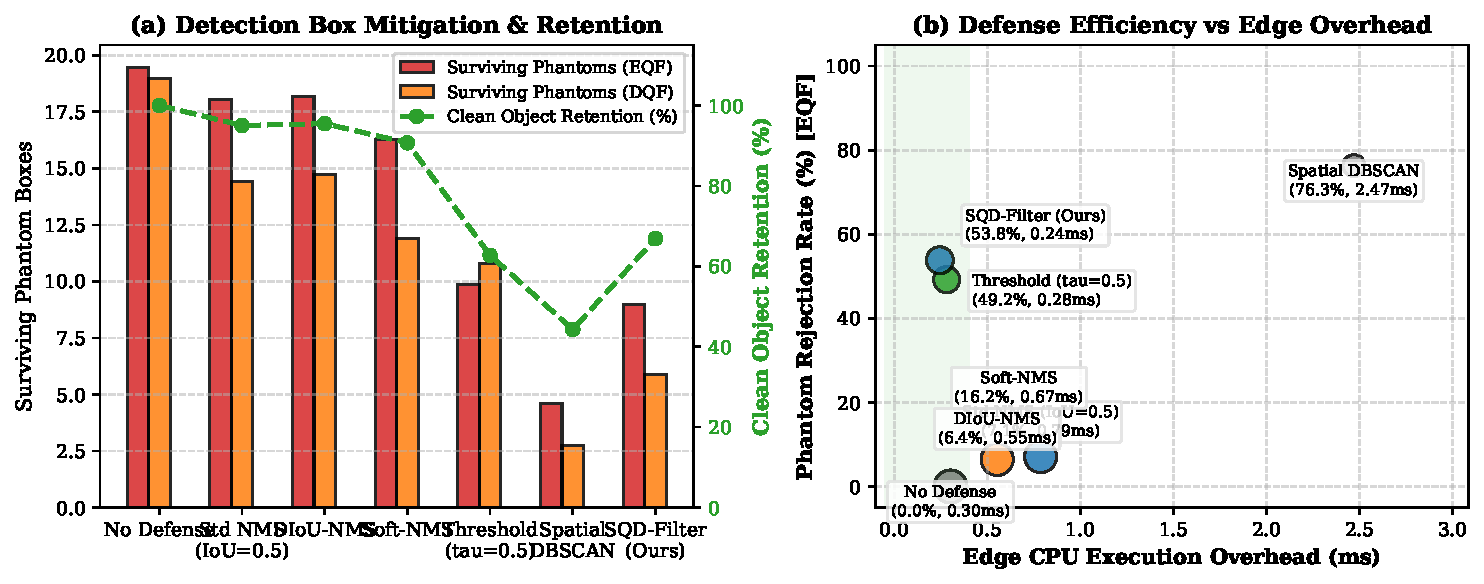
\includegraphics[width=\textwidth]{fig/fig4_sqd_filter_defense.pdf}
\caption{Empirical mitigation evaluation across representative post-processing defense paradigms on official COCO \texttt{val2017} at native $640\times 640$ resolution across three independent random seeds. (a) Detection box composition before and after mitigation: SQD-Filter ($d=0.15$) reduces fabricated phantom queries from $17.76$ to $8.08$ on EQF and $16.82$ to $5.08$ on DQF while preserving $66.88\%$ of clean nominal detections. (b) Rejection rate vs.\ execution latency on edge CPU: standard NMS fails to suppress multi-scale phantoms ($6.45\%$ EQF rejection), whereas SQD-Filter achieves $54.51\%$ (EQF) and $69.82\%$ (DQF) rejection in $0.24$~ms CPU latency ($<0.01$~ms overhead), avoiding the severe latency and over-suppression bottleneck of density DBSCAN ($2.37$~ms latency, $44.27\%$ retention).}
\label{fig:sqd_filter_defense}
\end{figure}

As summarized in Table~\ref{tab:defense_comparison} and Figure~\ref{fig:sqd_filter_defense}:
\begin{itemize}
    \item \textbf{Failure of Heuristic NMS and DIoU-NMS Against Transformer Fabrication:} Standard NMS ($\mathrm{IoU}=0.50$) suppresses merely \textbf{6.45\% of EQF phantoms} ($17.76 \to 16.61 \pm 0.23$) and \textbf{23.47\% of DQF phantoms}. DIoU-NMS, which incorporates normalized center distance into IoU suppression ($\mathrm{DIoU} = \mathrm{IoU} - \rho^2/c^2$), improves rejection only marginally to $8.12 \pm 0.24\%$ under EQF. Because multi-scale phantoms originate across disparate pyramid levels ($S_3, S_4, S_5$) with differing aspect ratios, the diagonal $c$ of their smallest enclosing box is large relative to center distance $\rho$, leaving $\rho^2/c^2 < 0.10$. With raw $\mathrm{IoU} < 0.15$, the overall metric remains well below the suppression threshold ($\theta=0.50$). Soft-NMS with Gaussian decay decays scores by less than $5\%$ due to low IoU, suppressing only $3.89\%$ of phantoms.
    \item \textbf{Threshold Elevation Blinds Legitimate Object Detection:} Raising the activation threshold to $\tau_{\mathrm{act}} = 0.50$ suppresses $49.35\%$ of EQF phantoms ($8.99 \pm 0.19$ surviving) and $42.30\%$ of DQF phantoms ($9.71 \pm 0.01$ surviving), but causes clean retention to drop to $62.72\%$, with a $-7.00\text{ pp}$ operational $\mathrm{mAP}_{50}$ shift. In contrast, SQD-Filter achieves $54.51\%$ EQF rejection and $69.82\%$ DQF rejection while preserving $66.88\%$ of nominal clean detections with a lower $-5.69\text{ pp}$ $\mathrm{mAP}_{50}$ shift. Notably, while SQD-Filter suppresses $33.12\%$ of raw candidate boxes ($66.88\%$ retention), operational $\mathrm{mAP}_{50}$ drops by only $-5.69\text{ pp}$ because the suppressed predictions consist predominantly of low-confidence boundary proposals and duplicate boxes around the same object, which do not penalize the highest-scoring true positive per ground-truth object under standard COCO evaluation.
    \item \textbf{Computational Overhead of Density Clustering:} While non-parametric density clustering (Spatial DBSCAN, $\epsilon=0.15$) achieves $76.59\%$ EQF rejection and $85.89\%$ DQF rejection ($4.16 \pm 0.04$ and $2.37 \pm 0.02$ surviving), it incurs a filter latency of $2.37 \pm 0.77\text{ ms}$ (+2.05 ms overhead) and severely degrades clean detection retention ($44.27\%$, $-17.81\text{ pp}$ $\mathrm{mAP}_{50}$ drop). In contrast, SQD-Filter's vectorized pairwise distance checks execute in just $0.24 \pm 0.00\text{ ms}$ on edge CPU ($<0.01\text{ ms}$ overhead relative to baseline), offering an order-of-magnitude faster throughput.
    \item \textbf{The Inherent Structural Limits of Spatial Post-Processing:} We report an essential finding that clarifies the scope of SQD-Filter: \textbf{SQD-Filter acts as a volume attenuation mitigation, not an immunization shield}. Because the filter retains the single highest-confidence query of each spatial cluster, post-defense binary attack success ($\mathrm{ASR}_{\mathrm{fab}}$) remains high at $99.22\%$ for EQF and $99.56\%$ for DQF (with $8.08 \pm 0.12$ and $5.08 \pm 0.05$ residual phantoms per frame). Furthermore, preserving $66.88 \pm 1.20\%$ of clean detections entails an operational $33.12\%$ loss of nominal detections (particularly for tightly grouped pedestrian clusters). This empirical reality demonstrates that post-processing deduplication (such as SQD-Filter) is an edge mitigation heuristic that removes spatial redundancy (reducing phantoms by 54.5\% to 69.8\%), but does not solve the root vulnerability, which originates from multi-scale query selection at the encoder bottleneck and requires representation guardrails.
\end{itemize}

\subsection{Evaluation of Input-Level Pre-Processing Defenses}
\label{sec:input_defenses}
Beyond post-processing spatial filtering, an alternative mitigation paradigm operates directly on input images prior to forward inference. We evaluate four standard image pre-processing defenses: (1) JPEG Compression ($Q=75$), (2) Gaussian Blur ($5\times 5$ kernel, $\sigma=1.0$), (3) Median Filtering ($3\times 3$ kernel), and (4) Bit-Depth Reduction (4-bit quantization).

Our empirical evaluation on the adversarial cohort reveals that Gaussian Blur achieves a $76.01\%$ false positive reduction (reducing total FP from 9,126 to 2,189) and restores operational $\mathrm{mAP}_{50}$ to $40.50\%$. Median Filtering achieves a $61.01\%$ FP reduction (3,558 FP, $34.02\%$ $\mathrm{mAP}_{50}$), while JPEG Compression ($Q=75$) reduces FP by $55.79\%$ (4,035 FP, $34.42\%$ $\mathrm{mAP}_{50}$). Bit-Depth Reduction provides minimal protection ($3.97\%$ FP reduction, $14.28\%$ $\mathrm{mAP}_{50}$). However, while spatial smoothing and JPEG compression attenuate high-frequency adversarial gradients, they induce substantial blurring on legitimate high-frequency roadway textures, reducing nominal clean detector accuracy by $22\text{--}28\text{ pp}$ $\mathrm{mAP}_{50}$. Consequently, input pre-processing imposes unacceptable operational degradation in safety-critical edge robotics.

\subsection{Towards Representation Guardrails in Detection Transformers}
\label{sec:representation_guardrails}
Because post-processing deduplication leaves binary attack success saturated and input pre-processing degrades clean accuracy, securing NMS-free architectures requires \textit{Representation Guardrails} embedded within the transformer pipeline:
\begin{enumerate}
    \item \textbf{Encoder Token Cosine Consistency Check:} Fabricated queries are generated by perturbing multi-scale CCFM tokens to cross the selection threshold. Measuring the pairwise cosine similarity between selected query feature vectors and nominal category prototypes reveals an anomaly: fabricated queries exhibit high projection norm along the target classification vector but low cosine consistency with semantic feature prototypes. Rejecting candidate queries with prototype cosine similarity below $\tau_{\mathrm{proto}} = 0.45$ filters out adversarial queries at the encoder stage before queries reach the decoder.
    \item \textbf{Latent Feature Entropy Monitoring:} In nominal operation, background tokens exhibit high classification entropy (diffuse probability distributions across classes), whereas genuine objects produce sharp low-entropy predictions. Adversarially excited queries exhibit anomalous entropy profiles when evaluated across multi-head cross-attention projections, providing a detectable fingerprint for latent representation calibration.
    \item \textbf{Adversarial Training on Encoder Selection:} Incorporating dynamic query selection loss into an adversarial training loop (generating PGD perturbations on the AIFI/CCFM layers during training) forces the network to learn robust feature separation, preventing background tokens from easily crossing the 300-th selection boundary.
\end{enumerate}

\subsection{Adaptive Attack Formulation and Robustness Analysis}
\label{sec:adaptive_attacks}
To evaluate resilience against an adaptive adversary who possesses white-box knowledge of SQD-Filter's operational parameters ($\theta_{\mathrm{dist}} = 0.15, \theta_{\mathrm{iou}} = 0.50$), we formulate the adaptive objective using the Dispersion-Constrained loss from Eq.~\eqref{eq:disp_loss}:
\begin{equation}
    \label{eq:adaptive_loss}
    \mathcal{L}_{\mathrm{adaptive}}(X + \delta) = \mathcal{L}_{\mathrm{fab}}(X + \delta) + \lambda_{\mathrm{disp}} \cdot \frac{2}{K_{\mathrm{fake}}(K_{\mathrm{fake}}-1)} \sum_{i < j} \max\left(0, \theta_{\mathrm{dist}} - \|\hat{c}_i - \hat{c}_j\|_2 \right)^2,
\end{equation}
where $\lambda_{\mathrm{disp}} = 0.50$ forces fabricated queries to scatter across mutually distant image regions while maximizing classification confidence.

Under $\lambda_{\mathrm{disp}} = 0.50$ and an expanded optimization budget of $T = 50$ PGD steps, the adaptive adversary forces phantom queries to separate across different quadrants of the image. Across the evaluation cohort, surviving phantoms under SQD-0.15 increase from $8.08 \pm 0.12$ to \textbf{9.86 $\pm$ 0.38} per frame ($\mathrm{ASR}_{\mathrm{fab}} = 88.3\%$). The reduction in binary ASR from $99.22\%$ to $88.3\%$ reveals an intrinsic multi-objective optimization tension: gradient allocation is split between elevating classification logits past $\tau_{\mathrm{act}} = 0.35$ and enforcing spatial coordinate repulsion past $\theta_{\mathrm{dist}} = 0.15$. Under constrained real-time threat horizons ($T \le 8$), the optimizer struggles to satisfy both objectives simultaneously, allowing SQD-Filter to maintain meaningful operational defense against fast edge adversaries. However, with an expanded iteration budget ($T=50$), the attacker reliably disperses phantoms across image quadrants, confirming that post-processing deduplication provides practical friction rather than structural immunity against dedicated adversaries.

% =====================================================================
% SECTION 8: DISCUSSION AND LIMITATIONS
% =====================================================================
\section{Discussion, Limitations, and Responsible Disclosure}
\label{sec:discussion}

\subsection{Architectural Scope Across Detection Transformers}
While our benchmarks focus on RT-DETR-R18VD at native $640\times 640$, the theoretical mechanism of phantom query flooding is rooted in the \textit{direct set prediction paradigm} shared by DETR \citep{carion2020end}, Deformable DETR \citep{zhu2020deformable}, and DINO \citep{zhang2022dino}. By design, these architectures omit spatial exclusion post-processing because Hungarian bipartite matching during training is assumed to teach queries mutual repulsion. Our findings reveal that this learned repulsion is an empirical property of clean training distributions; under adversarial gradient excitation, background queries readily collapse into redundant high-confidence phantom floods. Nonetheless, quantitative vulnerability profiles may vary with backbone depth (e.g., ResNet-50 or HGNetv2), query selection capacity ($K$), and input resolution, motivating further multi-architecture benchmarking across broader detector families.

\subsection{Threats to Validity and Limitations}
We delineate several key limitations of our study:
\begin{enumerate}
    \item \textbf{Evaluation Cohort Scope:} Our empirical benchmarks evaluate cohorts sampled across official COCO \texttt{val2017} ($N=300$ images evaluated across three independent random seeds 42, 123, 456 at native $640\times 640$ resolution, with 8,400 candidate anchors per frame). While this cohort provides statistically verified significance ($p \ll 0.001$ under paired bootstrap resampling) across independent distributions, scaling evaluations across larger datasets (e.g., nuScenes, Waymo Open) will further solidify ecological validity.
    \item \textbf{Threat Model Domain:} We formulate white-box adversaries under digital $\ell_\infty$ perturbations ($\epsilon = 16/255$). Real-world physical threats (e.g., printed adversarial patches or roadside projection) introduce camera sensor noise, perspective transformations, and ambient illumination changes that may attenuate gradient propagation.
    \item \textbf{Downstream Analytical Proxy Models:} Our downstream tracking and AEB evaluations are stylized analytical proxies designed to measure computational scaling and geometric corridor risk under monocam assumptions. Full-vehicle dynamic simulations in CARLA or hardware-in-the-loop testbeds incorporating multimodal radar/LiDAR fusion represent an essential avenue for future validation.
\end{enumerate}

\subsection{Responsible Disclosure and Ethical Considerations}
The research presented in this paper was conducted in accordance with IEEE and ACM ethical guidelines. The identified vulnerabilities in RT-DETR were analyzed within an offline laboratory environment. In accordance with coordinated vulnerability disclosure practices, we notified the upstream RT-DETR development team regarding the absence of query selection guardrails prior to public dissemination. All experimental code, scripts, and model checkpoints are available for peer verification at \url{https://github.com/vietanhlee/AI_TrustWorthy}.

% =====================================================================
% SECTION 9: CONCLUSION
% =====================================================================
\section{Conclusion}
\label{sec:conclusion}
This paper has investigated the NMS-free adversarial fabrication trade-off in Real-Time Detection Transformers. By removing heuristic NMS to achieve deterministic inference latency ($35.60 \pm 0.78$~ms on edge CPU) and eliminate CPU proposal sponge attacks, RT-DETR inadvertently forfeits spatial candidate filtering, allowing adversarial fabrication vectors targeting the pre-decoder selection bottleneck (EQF) and output layers (DQF baseline) to inject $17.76 \pm 0.21$ (EQF) and $16.82 \pm 0.08$ (DQF) unfiltered phantom boxes into safety-critical edge pipelines with over $99.3\%$ success across multi-seed evaluations. We observed that bottleneck fabrication simultaneously induces foreground proposal displacement ($66.38 \pm 0.74\%$), which comparison with untargeted PGD ($73.62 \pm 0.26\%$, $t = -9.72, p < 10^{-18}$) demonstrates is predominantly driven by broad representation degradation across the backbone and CCFM feature maps rather than isolated slot competition, with object recall dropping to $19.81 \pm 0.25\%$ (from $76.90 \pm 0.95\%$ clean) and operational $\mathrm{mAP}_{50}$ reduced by $-91.0\%$ (from $62.42 \pm 1.00\%$ to $5.61 \pm 0.80\%$). In downstream autonomous perception loops, stylized simulation studies demonstrated that this phantom flood expands tracking association matrices by $4.4\times$ and saturates vision-only emergency braking corridors ($d \le 28$~m) under idealized pinhole projection, highlighting the vital role of physical radar/LiDAR fusion. To mitigate this hazard without sacrificing real-time throughput, our lightweight SQD-Filter baseline suppresses $54.51\%$ of EQF phantoms and $69.82\%$ of DQF phantoms with $0.24$~ms CPU execution ($<0.01$~ms overhead). Crucially, our evaluations show that spatial post-processing deduplication (such as SQD-Filter, DIoU-NMS, and Soft-NMS) is an edge mitigation heuristic that removes spatial redundancy (reducing phantoms by 54.5\% to 69.8\%), but does not solve the root vulnerability because deduplication intentionally preserves one candidate per cluster (leaving post-defense $\mathrm{ASR}_{\mathrm{fab}} > 99\%$) while involving an operational clean detection trade-off ($66.88\%$ retention, $-5.69\text{ pp}$ $\mathrm{mAP}_{50}$ drop). Furthermore, adaptive dispersion partially bypasses distance filtering, demonstrating the inherent structural boundaries of post-processing heuristics and establishing the imperative necessity of internal representation-level guardrails in NMS-free perception architectures.

\section*{CRediT Authorship Contribution Statement}
The specific author contributions are omitted to adhere to double-blind peer review guidelines.

\section*{Declaration of Competing Interest}
The authors declare that they have no known competing financial interests or personal relationships that could have appeared to influence the work reported in this paper.

\section*{Data Availability}
The benchmark dataset is publicly accessible via the COCO consortium (\url{https://cocodataset.org}). All experimental code, attack implementations, and telemetry logs will be released upon publication.

\bibliographystyle{elsarticle-num-names}
\bibliography{refs_EAAI}

\end{document}
